\documentclass[a4paper,headsepline,bibtotocnumbered,12pt,titlepage,twoside]{scrartcl}

\usepackage[utf8]{inputenc}
\usepackage[T1]{fontenc}

\usepackage[english,ngerman]{babel}

\usepackage{graphicx}
\usepackage{upgreek}
\usepackage{float}
\usepackage{units}
\usepackage{url}

\usepackage{amsmath}
\usepackage{amssymb}
\usepackage{amsfonts}

\usepackage{longtable}

\usepackage[FIGTOPCAP,tight,raggedright,nooneline]{subfigure}
\usepackage[colorlinks=false, pdfborder={0 0 0}]{hyperref}

\usepackage[automark]{scrpage2}
\pagestyle{scrheadings}
\clearscrheadfoot
\ohead{\pagemark}
\ihead{\headmark}
\usepackage{setspace}
\linespread{1.25}
\usepackage{geometry}
%~ \geometry{a4paper, top=21mm, left=30mm, right=30mm, bottom=21mm,
          %~ headsep=10mm, footskip=12mm}
\geometry{a4paper, top=21mm, bottom=21mm, headsep=10mm, footskip=12mm}

\addtokomafont{sectioning}{\rmfamily}
\usepackage[bf]{caption}
\captionsetup{format=plain}
\setlength{\parindent}{0pt}
\fussy

\newcommand{\change}[1]{{#1}}

\usepackage{ae}
\usepackage{booktabs}

%\abs{Ausdruck} %Betragsstriche, die skalieren - abgekürzt
\newcommand{\abs}[1]{\ensuremath{\left\vert#1\right\vert}}
% und das gleiche füur große Klammern
\newcommand{\brac}[1]{\ensuremath{\left(#1\right)}}
% Erwartungswert skalierend
\newcommand{\avg}[1]{\left< #1 \right>}
% ein nicht kursives d für Ableitungen/Integrale, mit etwas Platz davor, um sich etwas abzusetzten
\newcommand{\de}{\ensuremath{\,\mathrm{d}}}
% Für Einheiten: schreibt sie nicht kursiv und lässt etwas Platz zur Zahl vorher
\newcommand{\eh}[1]{\ensuremath{\,\mathrm{#1}}}
% einfaches Gradzeichen
\newcommand{\gr}{\ensuremath{^{\circ}}}
% Fehlerfortpfanzung
% dy/dz * delta z
\newcommand{\fehler}[2]%
{\ensuremath{\abs{\frac{\partial #1}{\partial #2}}\cdot \Delta #2}}

\hyphenation{}
\setcounter{lofdepth}{2}

\numberwithin{equation}{section}
\numberwithin{figure}{section}
\numberwithin{table}{section}

\begin{document}
    \selectlanguage{ngerman}
    \begin{titlepage}
\begin{center}


\includegraphics[width=90mm]{images/Uniol_1c.pdf}\\
\vspace{25mm}

{\LARGE  Bachelorarbeit im Fach Physik\\}

\vspace{10mm}

{\LARGE \bfseries
Ising-Ferromagnet auf Ad-Hoc Netzwerken
\\}

\vspace{20mm}

\begin{minipage}{0.4\textwidth}
\begin{center} \large
\emph{von}\\
\large
Hendrik Schawe\\
\end{center}
\end{minipage}

\vspace{45mm}

{\large
Betreuender Gutachter:\\
Prof.\ Dr.\ Alexander K. Hartmann\\
}
\vspace{8mm}
{\large
Zweitgutachter:\\
Dr.\ Oliver Melchert\\
}

\vfill
{\large Oldenburg, den 05.\ Juni 2013}
\newpage

\end{center}

\end{titlepage}

    \selectlanguage{english}
    \thispagestyle{empty}
    \cleardoublepage
    \setcounter{page}{1}
    \pagenumbering{roman}
    \tableofcontents
    \newpage
    \listoffigures
    \listoftables

    \clearpage
    \pagestyle{empty}
    \cleardoublepage
    \pagestyle{scrheadings}


    \setcounter{page}{1}
    \pagenumbering{arabic}

    \section{Introduction}
        The computing capabilities of modern computers enable researchers to
collect and analyze vast amounts of data. The prime example for this fact
is the LHC, where petabytes of particle collision data are collected,
processed and discarded or kept every second \cite{LHC}.
But computers are not only able to process measured data, but
also to generate data by simulations of, e.g., statistical systems, where
the rules for each subsystem are well defined but the behavior of the
whole system is not easy to predict because of the nontrivial interactions of the
subsystems. For those systems there often exists no analytic solution
or only for very simplified or special cases. But one can simulate all
the interactions of the subsystems and observe the behavior of the whole
system using computational experiments.
For example one can examine phase transitions, which are defined by the abrupt
change of an observable, e.g., the change of the density of water near
boiling, which is liquid at \(T < T_c\) and gaseous at \(T > T_c\). Also
the change of the magnetization of a ferromagnet near the Curie temperature
is a phase transition from ferromagnetic at \(T < T_c\) to paramagnetic at \(T > T_c\).
This can be observed by heating some refrigerator magnet by a candle --
after this treatment it will no longer stick on the refrigerator.
Different phases of a material and the transitions between them were
always of greatest interest. The ancient Greek thought that everything
consists of fire, water, air and earth, which are the archetypes of
phases. Still phase transitions are important phenomenons, because they
are ubiquitious. The understanding allows applications from the
refrigerator to shatter resistant mobile phone glass \cite{PJournalGlass}.
There are different kinds of phase transitions which are distinguished by
the behavior of their order parameter and characterized by a set of
critical exponents \cite{yeomans}. If it shows a discontinuity at
the phase transition, it is a \emph{first order} phase transition, e.g.\ Water at boiling.
A \emph{second order} phase transition is characterized by a continuous
transition without discontinuities of the order parameter but a discontinuity
in its first derivative.\\
One of the simplest models with a second order phase transition is the
Ising model \cite{Ising1925} in \(d \ge 2\) dimensions. This is a simple
model of a ferromagnet and will be explained in more detail in Sec.\
\ref{ssec:isingmodel}. It is analytically solved in two dimensions on
some regular lattices \cite{Onsager1944} \cite{Wannier1945}.
In this thesis its behavior near the critical temperature -- also called
Curie temperature -- and the behavior of the critical temperature itself
on some irregular lattices corresponding to proximity graphs
(see Sec.\ \ref{ssec:graphtypes}) will be examined using the Monte
Carlo simulations described in Sec.\ \ref{ssec:montecarlo}.\\
Proximity graphs are canditates for ad-hoc networks. As an example of an
ad-hoc network take a wifi network without central devices, but every
participant (e.g.\ a laptop) works as a relay to get a data package to its
destination. To minimize the needed energy the packages will be routed
over small distances from one node to another. This behavior is well mapped
by proximity graphs. They establish a lattice by connecting sites which
are "near" to each other. The exact definition of "near" is dependend on
the proximity graph.\\
Because the Ising model on a regular square lattice is well understood,
the here investigated irregular lattices will be constructed starting from
a square lattice and displacing the sites governed by a parameter \(\sigma\).
Then the influence of \(\sigma\) on the critical temperature will be
analyzed. A crossover of the critical temperature from the square lattice
to the corresponding proximity graph is expected.\\

Unfortunately the memory of any computer is small in comparison to what
would be needed for a simulation of a system in the
thermodynamic limit. So only a very small number of elementary subsystems can be
simulated in comparison to the actual number of elementary subsystems
of the system in nature. This leads to deviations from the real behavior
of the system in the thermodynamic limit. These deviations are called
\emph{finite-size effects} and in Sec.\ \ref{ssec:finitesize} will be
discussed how to manage them.\\

Note that in the scope of this thesis the Boltzmann constant is \(k_{B}=1\)
for the sake of simplicity.


    \section{Model}
        %~ \subsection{Model and Implementation}
%~ I will desribe the model in this section in a bottom-up fashion.
%~ First describing all parts and then connecting them.

%~ \subsubsection{Graphs}
    %~ A graph is a set of nodes \(V\) and edges \(E\).
\subsection{Gabriel- and Relative Neighborhood Graph}
\label{ssec:graphtypes}
    A graph \(G(V,E)\) is a set of nodes \(V\) and edges \(E\).\\
    All here mentioned graph types are \emph{proximity graphs}. They are
    connecting nodes which are by some metric near to each other.
    Hence they are suited to generalize problems defined on regular
    lattices with nearest neighbor relationships, like the Ising model
    which will be described in more detail in section
    \ref{ssec:isingmodel}.
    In this thesis the distance is always determined by the Euclidian
    metric, though in principle every metric can be used.\\

    The Gabriel graph \cite{Gabriel1969} is a subgraph of the
    Delaunay triangulation. Two nodes \(i\) and \(j\) with distance
    \(d_{ij}\) are connected with an edge if a circle with it's
    center on the middlepoint between \(i\) and \(j\) and radius
    \(r = \frac d 2\) contains no other nodes. This area will be
    called \emph{lune} in the following. See also Figure
    \ref{fig:lunes}\subref{sfig:lunes:def}.\\
    The Relative Neighborhood graph \cite{Toussaint1980} is a
    subgraph of the Gabriel graph. Two nodes \(i\) and \(j\) with
    distance \(d_{ij}\) are connected if no other node is in the
    \emph{lune}. The lune is defined as the intersection of two
    circles with radius \(r = d\) and centers on \(i\) and \(j\).
    See also Figure \ref{fig:lunes}\subref{sfig:lunes:def}.
    \begin{figure}[htbp]
        \centering
        \subfigure[Definition of the lunes][]{
            \label{sfig:lunes:def}
            \tikzset{
    hatch distance/.store in=\hatchdistance,
    hatch distance=10pt,
    hatch thickness/.store in=\hatchthickness,
    hatch thickness=2pt
}

\makeatletter
\pgfdeclarepatternformonly[\hatchdistance,\hatchthickness]{flexible hatch no}
{\pgfqpoint{0pt}{0pt}}
{\pgfqpoint{\hatchdistance}{\hatchdistance}}
{\pgfpoint{\hatchdistance-1pt}{\hatchdistance-1pt}}%
{
    \pgfsetcolor{\tikz@pattern@color}
    \pgfsetlinewidth{\hatchthickness}
    \pgfpathmoveto{\pgfqpoint{0pt}{0pt}}
    \pgfpathlineto{\pgfqpoint{\hatchdistance}{\hatchdistance}}
    \pgfusepath{stroke}
}
\makeatletter
\pgfdeclarepatternformonly[\hatchdistance,\hatchthickness]{flexible hatch nw}
{\pgfqpoint{0pt}{0pt}}
{\pgfqpoint{\hatchdistance}{\hatchdistance}}
{\pgfpoint{\hatchdistance-1pt}{\hatchdistance-1pt}}%
{
    \pgfsetcolor{\tikz@pattern@color}
    \pgfsetlinewidth{\hatchthickness}
    \pgfpathmoveto{\pgfqpoint{0pt}{\hatchdistance}}
    \pgfpathlineto{\pgfqpoint{\hatchdistance}{0pt}}
    \pgfusepath{stroke}
}

\begin{tikzpicture}
    \clip (-2,2.25) rectangle (2,-1.75);

    \begin{scope}
        \clip (-1, 0.5) circle(2.06155281281);
        %~ \fill[fill=blue!20] (1, 0) circle(2.06155281281);
        %~ \draw[pattern=north west lines] (1, 0) circle(2.06155281281);
        \draw[pattern=flexible hatch no,hatch distance=10pt,hatch thickness=0.7pt] (1, 0) circle(2.06155281281);
    \end{scope}

    %~ \fill[fill=white] (0, 0.25) circle(1.0307764064);
    %~ \draw[pattern=north east lines] (0, 0.25) circle(1.0307764064);
    \draw[pattern=flexible hatch nw,hatch distance=10pt,hatch thickness=0.7pt] (0, 0.25) circle(1.0307764064);
    \draw[thick] (0, 0.25) circle(1.0307764064);

    \draw[thick] (-1, 0.5) circle(2.06155281281);
    \fill (-1, 0.5) circle(0.1);
    \draw[thick] (1, 0) circle(2.06155281281);
    \fill (1, 0) circle(0.1);
    \draw[thick] (1, 0) -- (-1, 0.5);
\end{tikzpicture}

        }
        \subfigure[Relative Neighborhood graph example][]{
            \label{sfig:lunes:rng}
            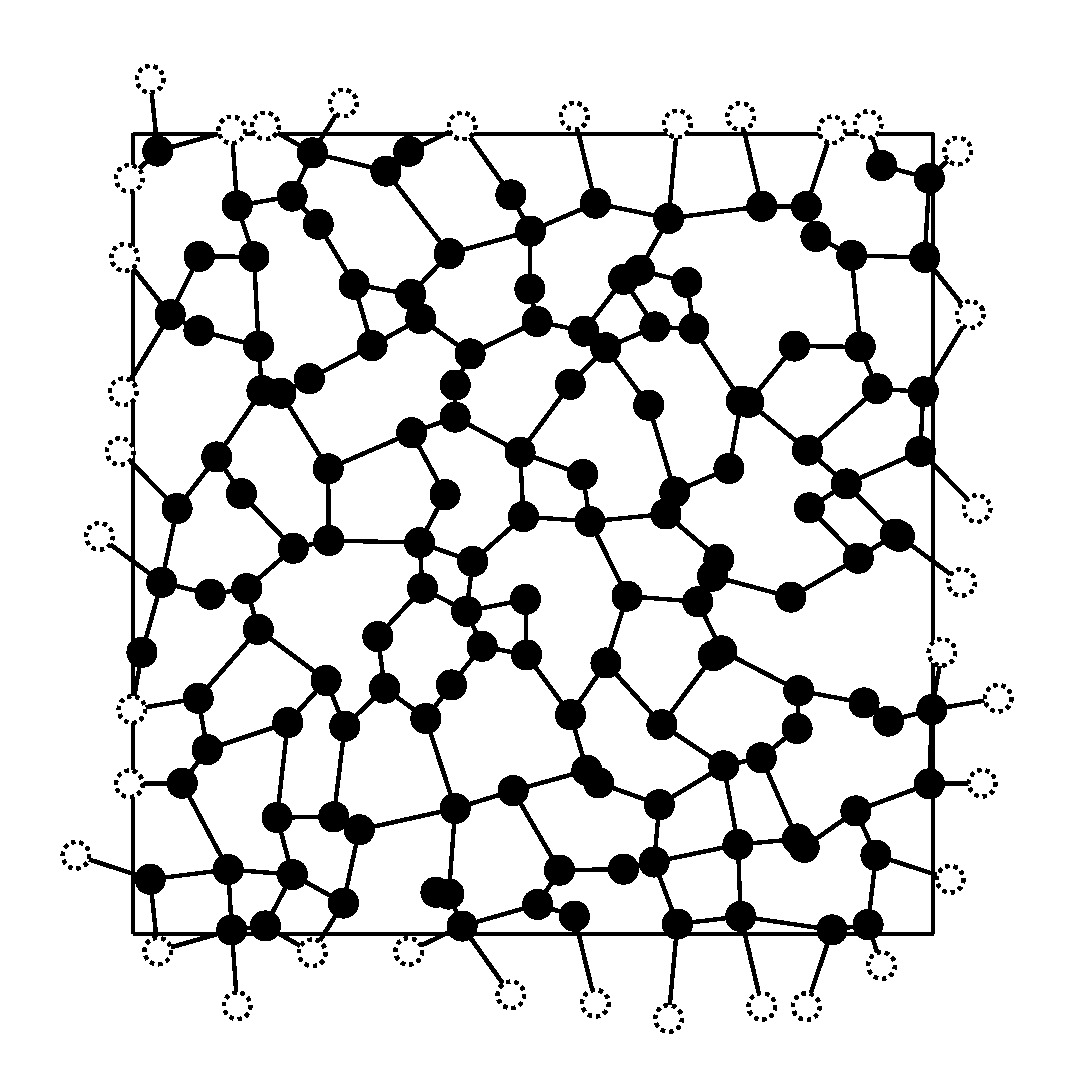
\includegraphics[width=0.3\textwidth]{images/RNG/L12S03.pdf}
        }
        \subfigure[Gabriel graph example][]{
            \label{sfig:lunes:gg}
            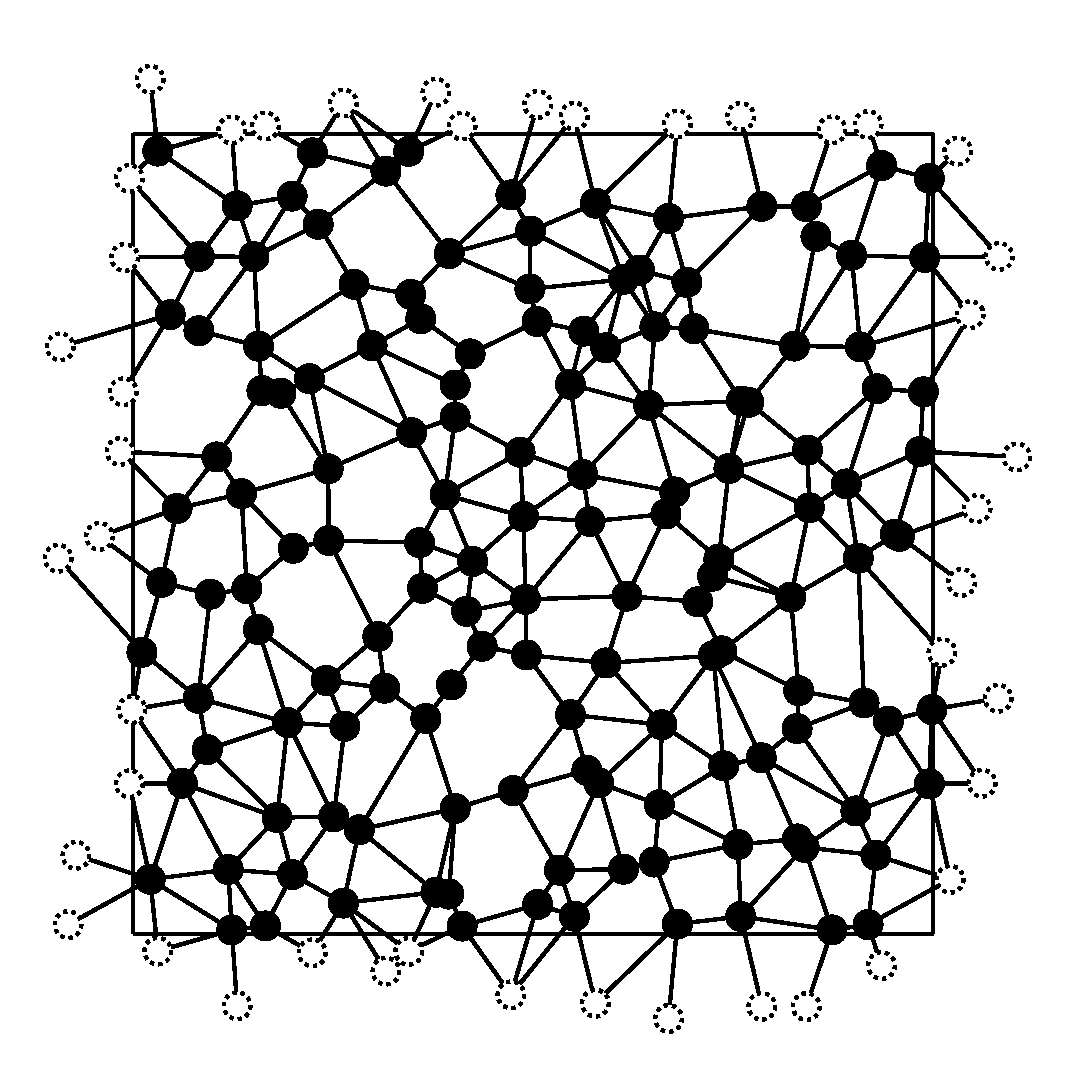
\includegraphics[width=0.3\textwidth]{images/GG/L12S03.pdf}
        }
        \caption[Gabriel - and Relative Neighborhood Graph]
        {
            \subref{sfig:lunes:def} Lunes of Relative Neighborhood
                Graph (hatched region) and
                Gabriel Graph (cross hatched region)
            \subref{sfig:lunes:rng} Example of a Relative
                Neighborhood Graph on periodic boundary conditions.
                Periodic nodes are dashed.
            \subref{sfig:lunes:gg} Example of a Gabriel Graph on
                periodic boundary conditions. Periodic nodes are
                dashed.
        }
        \label{fig:lunes}
    \end{figure}\\
    To construct these graphs the simple way is to test for each
    pair of nodes one has to check for every other node if it lies in
    the lune of the pair. That is of complexity \(O (N^3)\), because
    there are \(N(N-1)\) pairs and for each \(N-2\) nodes to test. So
    the product is of order \(O(N^3)\)\\
    To reduce the complexity one can first create a Delaunay
    Triangulation in complexity \(O (N \log N)\)
    \cite{Leach1992} and test the criterion for each edge, because
    the Delaunay triangulation is a supergraph of both. But the
    implementation of a Delaunay triangulation algorithm is not trivial
    and the generation of the graphs is not time critical in the scope
    of this bachelor thesis.\\
    So a tradeoff is to use basicly the simple method but only test
    the criterion for nodes which are near to the lune and abort if
    one node inside the lune is found. To determine which nodes are
    near the lune one can subdivide the area in \emph{cells} and save
    for each cell a list with nodes lying inside it like presented in
    \cite{RNGCell}.
    Now it is just neccessary to test the nodes in the cells which
    resemble a rectangular bounding box of the lune. Most pairs will be
    far away from each other and the cells in the middle of the bounding
    box are completely inside the lune so that only one node has to be
    tested to discard an edge between them. Connected nodes are near to
    each other so that only very few cells have to be tested.\\
    Indeed this method reduced the time needed to construct a Relative
    Neighborhood graph with \(N=32^2\) and \(N=64^2\) by a factor of
    over \(15\) respectivly \(40\). Though the complexity is still of
    order \(O(N^2)\) in the best case, because for every pair at least
    one check has to be performed.

\subsection{The Disordered Ising Model}
\label{ssec:isingmodel}
    The examined model is a modified 2D Ising model where the \(N=L^2\)
    sites are displaced nodes of a square lattice of edge length \(L\)
    with periodic boundary conditions. The displacement is randomly gauss
    distributed with the standard deviation \(\sigma\). This \(\sigma\)
    is also called \emph{disorder paramter} in the following.
    \begin{equation}
        \hat{H} = \sum_{\avg{i,j}}J_{ij}s_{i}s_{j} - H \sum_i s_i
        \label{eq:hamiltonian}
    \end{equation}
    Equation \eqref{eq:hamiltonian} is the hamiltonian of the Ising model.
    The magnetic field \(H=0\) in the scope of this thesis.
    \(\avg{i,j}\) refers to nodes \(i\) and \(j\) connected by an edge \(E_{ij}\).
    The edges are constructed according to one of the two the in section
    \ref{ssec:graphtypes} defined rules. So that the lattice represents
    a proximity graph. Each node \(i\) has a spin \(s_i = \pm 1\). Each
    edge \(E_{ij}\) has a weight \(J_{ij} = \exp (\alpha (1-d_{ij}))\).
    \(d_{ij}\) is the Euclidian distance between the nodes \(i\) and
    \(j\) and \(\alpha = 0.5\). \(J\) is called \emph{coupling constant}.\\
    For \(\sigma = 0\) this is the standard Ising model with \(J = 1\),
    for which exists an analytical solution \cite{Onsager1944}.\\

    For evaluation the Monte Carlo simulation is is run till the system
    is equilibrated after \(t_{eq}\) sweeps. Then the simulation continues
    and the magnetisation per site \(m\) and energy per site \(E\)
    are calculated and saved for every \(2\tau\) sweeps. Where \(\tau\)
    denotes the \emph{autocorrelation time} (see also \ref{ssec:eqtime}).
    For every observable \(O\) the expected value \(\avg{O}\) is determined
    as the mean of \(10000\) measurements for \(L=16,32\) or \(5000\) for
    \(L=64,128\). The expected values \(\avg{O}\) for \(100\) different
    random proximity graphs with the same disorder paramter \(\sigma\)
    are then averaged to \(\overline{\avg{O}}\). The errors are estimated
    by bootstrapping.

\subsection{Critical Temperature $T_c$ and Critical Exponents}
\label{ssec:finitesize}
    The aim of this thesis is to find the critical temperature \(T_c\)
    of the disordered Ising model in dependence of the disorder parameter
    \(\sigma\). At \(T_c\) the mean absolute magnetisation \(\avg{|m|}\) of
    the system will jump and the susceptibility
    \(\chi = \frac{N}{T}\brac{\avg{m^2}-\avg{m}^2}\)
    will diverge. In fig. \ref{fig:smeared_out}\subref{sfig:smeared_out:meanM}
    it is easy to see that the jump occurs at lower temperatures \(T\) for higher
    disorder parameters \(\sigma\) (here with a Relative Neighborhood graph).
    \begin{figure}[htbp]
        \centering
        \subfigure[Dependence of the phase transition on $\sigma$][]
        {
            \label{sfig:smeared_out:meanM_L}
            \includegraphics[width=0.45\textwidth]{plots/Mean_M_L_128}
        }
        \subfigure[Example for finite size effects][]
        {
            \label{sfig:smeared_out:meanM}
            \includegraphics[width=0.45\textwidth]{plots/meanM}
        }
        \caption[Phase Transition and Finite Size Effects]
        {
            \subref{sfig:smeared_out:meanM_L}: Effects of the disorder
            parameter $\sigma$ on the phase transition
            for an underlying Relative Neighborhood graph with $L=128$.\\
            \subref{sfig:smeared_out:meanM}: Effects of different system
            sizes at \(\sigma = 0\). Dotted lines are guides to the eye.
        }
        \label{fig:smeared_out}
    \end{figure}\\
    But in the shown plots there occurs no real jump, but a continuous
    decline. The jump is only present in infinite systems, hence every
    computer simulation will show some \emph{finte size effects}.
    These finite size effects cause a "smearing out" of the phase
    trasition. This is stronger for smaller system sizes, as is visible
    in fig. \ref{fig:smeared_out}\subref{sfig:smeared_out:meanM}. Clearly
    the \(L=16\) curve is much less steep than the \(L=128\) curve.\\
    Despite of this one can obtain \(T_c\) by finite size scaling
    methods \cite[S. ??]{NewmanBarkema1999} which also yield the critical
    exponents.
    Studies on random lattices with variing coupling constants \(J\)
    \cite{Lima2000} and without \cite{Janke1994} suggest, that the
    critical exponents should not be influenced by the disorder paramter
    \(\sigma\). So they will be used for consistency cross checking and
    comparision with the known exact values \cite[S. 59]{Pelissetto2002}.\\
    It is known, that for large \(L\) near the critical temperature the
    equations \eqref{eq:fsscaling:m}, \eqref{eq:fsscaling:chi} and
    \eqref{eq:fsscaling:g} apply \cite[p. 145f]{Katzgraber2011}.
    \begin{align}
        \label{eq:fsscaling:m}
        \avg{m_L} &= L^\frac{\beta}{\nu} \tilde{M}\brac{L^\frac{1}{\nu}\brac{T-T_c}}\\
        \label{eq:fsscaling:chi}
        \chi_L    &= L^\frac{\gamma}{\nu} \tilde{C}\brac{L^\frac{1}{\nu}\brac{T-T_c}}\\
        \label{eq:fsscaling:g}
        g         &\propto \tilde{G}\brac{L^\frac{1}{\nu}\brac{T-T_c}}
    \end{align}
    Where \(g = 3-\frac{\avg{m^4}}{2\avg{m^2}^2}\) \cite{Binder1981} is
    the Binder cumulant and \(\tilde{M}, \tilde{C}\) and \(\tilde{G}\)
    are unkown scaling functions. To find the exponents
    \(\beta, \gamma, \nu\) and the critical temperature \(T_c\), one
    varies them until the measured values of the observables collapse on
    one curve. Like the obersables from fig. \ref{fig:gettingCrit}\subref{sfig:gettingCrit:binder_fit_s_0}
    collapse in fig. \ref{fig:gettingCrit}\subref{sfig:gettingCrit:collapse_s_0}.
    Note that \(L=16\) is not used for the collapse, because it is a
    rather small value such that eq. \eqref{eq:fsscaling:m}-\eqref{eq:fsscaling:g}
    do not apply very good.\\
    To accomplish the collapse in an semi-automatic and reproduceable
    way with an error estimate, the programm
    \texttt{autoscale.py} \cite{autoscale2009} is used.
    \begin{figure}[htbp]
        \centering
        \subfigure[Example of a Binder cumulant to determine the critical temperature][]{
            \label{sfig:gettingCrit:binder_fit_s_0}
            \includegraphics[width=0.47\textwidth]{plots/binder_fit_s_0}
        }
        \subfigure[Example of a datacollapse to determine critical exponents][]{
            \label{sfig:gettingCrit:collapse_s_0}
            \includegraphics[width=0.47\textwidth]{plots/collapse_s_0}
        }
        \caption[Examples of determining critical temperature and exponents]
        {
            The Binder cumulant \(g\) of an square lattice Ising model
            (\(\sigma=0\))\\
            \subref{sfig:gettingCrit:binder_fit_s_0} interpolated
                with cubic splines (the errorbars are too small to see)\\
            \subref{sfig:gettingCrit:collapse_s_0} collapsed by finite
                size scaling
        }
        \label{fig:gettingCrit}
    \end{figure}\\
    Though if one is just interested in the critical Temperature, an
    easier approach is to find the intersections of the Binder cumulants
    \(g\) of different system sizes \(L\) because they are intersecting
    at \(T_c\) \cite{Binder1981}.
    Therefore a cubic spline interpolation\footnote{created using the \texttt{scipy.interpolate} tools \cite{scipy2001}}
    is calculated for the measured points.
    As an example take fig. \ref{fig:gettingCrit}\subref{sfig:gettingCrit:binder_fit_s_0}.
    Here such interpolations are plotted for \(\sigma=0\) and are
    intersecting at \(\approx 2.27\).
    To determine \(T_c\) the intersections\footnote{found using the \texttt{scipy.optimize} tools \cite{scipy2001}}
    are averaged and the standard error is calculated. In this case one
    gets \(T_c = 2.2689(2)\), which is in good agreement with the
    exact solution from eq. \eqref{eq:exactTc} \cite{Onsager1944}.
    \begin{equation}
        T_c = 2J/\ln(1+\sqrt 2) = 2.2691...
        \label{eq:exactTc}
    \end{equation}

% Erwahnen, dass T_c Graph so aussieht, wie degree graph
% mit theo ergebnissen von Honeycomb \cite{Wannier1945} vergleichen (fur deg = 3)
% cosh(2L_c)=2 mit L_c = J/2kT_c -> T_c \approx 1.52


    \section{Methods}
        \subsection{Thermodynamic Theory}
\label{ssec:theory}
    The disordered Ising model will be examined as a \emph{canonical system} in
    \emph{equilibrium}. A canonical system can exchange energy with a
    heat bath, thus it has a constant temperature equal to the temperature of the
    heat bath.
    Equilibrium is defined as a steady state, wherein
    the observables are only fluctuating but not changing in any
    particular direction. For example thermal equilibrium denotes the
    condition that the system under scrutiny has reached the temperature
    of the heat bath. This is the case once no net energy exchange occurs,
    thus the energy of the simulated system reaches a steady state, where
    only fluctuations occur.
    In a canonical ensemble the probability \(p_\nu\) of a state
    \(\nu\) is distributed according to a Boltzmann distribution
    \begin{equation}
        p_\nu = \frac{1}{Z} e^{-\beta H_\nu}
    \end{equation}
    \begin{equation}
        \beta = \frac{1}{k_B T}
    \end{equation}
    Where \(Z\) is the partition function, which normalizes \(p_\nu\) to
    a probability: \(\sum_\nu p_\nu = 1\).
    Further the free energy \(F\) of a canonical ensemble is minimized
    in equilibrium and all observables can be derived from \(F\)
    in a straight forward way, as stated in every textbook about
    statistical physics (e.g.\ Ref.\ \cite{nolting2005}).\\
    Because of
    \begin{equation}
        F = U - TS
    \end{equation}
    where \(S\) is the entropy, \(U=\avg{H}\) the internal energy and
    \(\avg{\cdot}\) declares the expectation value of an observable.
    One can guess that for low \(T\) the internal energy
    will be low, and for high \(T\) the entropy will be high to minimize
    \(F\).
    Considering the Hamiltonian of the Ising model, a spin configuration
    of high order, where most spins are aligned with their neighbors,
    leads to a low value of \(H\) and therefore a low value of \(U\).
    Simultaneously, this state of high order corresponds to a low entropy \(S\).
    Analogically a state of high \(U\) is also a state of high \(S\).
    These preliminary considerations make a phase transition at some
    \(T\) where the influence of the entropy on \(F\) becomes the same
    order of magnitude as the influence of the internal energy on \(F\),
    very plausible.\\
    To determine
    \begin{equation}
        F=-k_{B}T \ln{Z}
    \end{equation}
    one has to know the partition function
    \begin{equation}
        Z = \sum_\nu e^{-\beta H_\nu},
        \label{eq:partitionFunction}
    \end{equation}
    where the sum goes over all possible states \(\nu\) of the system.
    Then averages can be computed according to
    \begin{equation}
        \avg{O} = \frac{1}{Z} \sum_\nu O_\nu e^{-\beta H_\nu}.
    \end{equation}
    Because every site can have two states, there are \(2^N\) different
    states of the system. For each the energy \(H_\nu\) has to be calculated
    to solve the sum from Eq.\ \eqref{eq:partitionFunction} to gain \(Z\).
    Hence for small \(N\) the partition function is computable, but the system
    may show very different properties than in the thermodynamic limit.
    To minimize these finite size effects it is desirable to examine
    systems with large \(N\). But \(2^N\) is a very rapidly increasing
    number, so for large \(N\) it is unfeasible to calculate the energy for each state, except
    for cases where it is possible to solve it analytically.\\
    If not, one can get estimates of the observables for big \(N\) using
    Monte Carlo simulations, which are introduced in the next chapter.\\

    The observables which are measured in this thesis are the
    magnetization per spin
    \begin{equation}
        m = \frac{1}{N} \sum_i s_i
    \end{equation}
    and the energy per spin
    \begin{equation}
        E = \frac{1}{N} H.
    \end{equation}
    As mentioned before, properties near the phase transition and the
    critical temperature \(T_c\), where the phase transition occurs, will
    be examined. The Ising system in two dimensions shows a second order
    phase transition, hence \(m\) and \(E\) are continous, but show at
    \(T_c\) an infinitly sharp slope in the thermodynamic limit, i.e.\
    the first derivative diverges.
    From statistical physics (See Ref.\ \cite{nolting2005}) it is known that
    these derivatives can be expressed by fluctuations, e.g.\ the specific
    heat can be expressed as
    \begin{equation}
        c = \frac{\partial \avg{H}}{\partial T} = k_B \beta^2 \avg{\brac{H-\avg{H}}^2}.
    \end{equation}
    The specific heat is a measure for how much energy is needed to change
    the temperature of the system.
    Analogically the susceptibility
    \begin{equation}
        \chi = N \beta \avg{\brac{m-\avg{m}}^2}
    \end{equation}
    is a measure for how strong an outer magnetic field changes the
    magnetization of the system.
    Beside these observables from classical physics, a fifth observable
    the Binder cumulant \cite{Binder1981}
    \begin{equation}
        g = \frac{3}{2}\brac{1-\frac{\avg{m^4}}{3\avg{m^2}^2}}
        \label{eq:binder}
    \end{equation}
    is considered.
    This is a dimensionless value, which can be used to determine the
    critical point. These five observables will be sufficient to analyse
    the phase transition in the scope of this bachelor thesis. All of them
    can be easily computed when \(m\) and \(E\) are measured. The next
    chapter will show, how to get estimates for them through Monte Carlo
    simulations.

\subsection{Monte Carlo Simulations}
\label{ssec:montecarlo}
    The idea behind Monte Carlo simulations is to take random samples of
    the observable, which should be measured, and to estimate the mean of
    the observable from this samples. To apply this technique to statistical
    ensembles, one creates sample states of the system, measures the
    observables and calculates the expected value through averaging.\\
    In statistical physics the expected value of an observable \(O\)
    is -- as also noted above -- calculated by
    \begin{equation}
        \avg{O} = \frac{1}{Z} \sum_\nu p_\nu O_\nu.
        \label{eq:estim}
    \end{equation}
    It is however possible that there are few states contributing
    massively more than others. In canonical systems at low \(T\)
    states with low values of \(H\) contribute much more than states with
    high values of \(H\).
    But if one samples the \(2^N\) states evenly, it is probable to miss
    them. This is called \emph{simple sampling} and results in large
    errorbars for any observable.
    It is therefore desirable to sample only the states with high
    contributions to the sum.
    As noted before, the system under scrutiny is canonical and therefore
    \(p_\nu\) is known. The states are distributed according to the Boltzmann
    distribution. Hence \emph{Importance Sampling} can be utilized.\\
    Instead of sampling uniformly distributed random states, one should sample
    states according to their occurence probability given by the Boltzmann
    distribution. In fact this reduces the estimator Eq.\ \eqref{eq:estim} to
    \begin{equation}
        O_M = \frac{1}{M} \sum_{\nu=1}^M O_\nu,
    \end{equation}
    where \(M\) is the number of samples. The proof is shown in \cite{NewmanBarkema1999}.
    This is a very convenient form.\\
    But it is difficult to create a random state of a physical system,
    e.g.\ the Ising system, according to a given distribution. The simple
    approach of creating uniformly distributed random states and reject
    them with probability \(p_\nu^{-1}\) depending on their energy is not
    efficient, because many generated states will be discarded and the
    computing time to generate them and calculating their energy will
    be wasted.
    Hence one uses \emph{Markov Chains} to generate new states \(\nu\)
    from former ones \(\mu\). It is important that the transition probabilities
    \(A(\mu \to \nu)\) obey \emph{Detailed Balance} and \emph{Ergodicity}.
    \emph{Detailed Balance} means that the probability to leave a state is
    the same as the probability to enter the state in equilibrium
    \(p_\mu A(\mu \to \nu) = p_\nu A(\nu \to \mu)\) with \(p_\mu\) the
    probability to be in state \(\mu\).
    \emph{Ergodicity} requires that every possible state is reachable
    from every other state in finite time, see Refs.\ \cite{NewmanBarkema1999} \cite{Katzgraber2011}.
    This ensures that the system can equilibrate and that the states are
    distributed according to the desired distribution in equilibrium
    \cite{NewmanBarkema1999}. Otherwise the samples might not be representative
    for the whole system.\\
    In this thesis three algorithms, which fulfill all requirements,
    were used. They will be shortly described in the following subsections.
    But first equilibration- and autocorrelation time will be discussed.

    \subsubsection{Equilibration- and Autocorrelation Time}
    \label{sssec:eqtime}
        To generate states acoording to the Boltzmann distribution at a
        given temperature \(T\), one starts with an arbitrary state
        and waits until it reaches thermal \emph{equilibrium}. Because
        equilibrium is defined as a steady state, one can determine it by
        observing the change of the observables over the progressing
        simulation as pictured in Fig.\ \ref{fig:equiandauto}\subref{sfig:equiandauto:equiE}.
        The progression of a Monte Carlo simulation is measured in \emph{sweeps},
        which denote some operation. The count of sweeps until
        equilibrium is reached, is called \emph{equilibration time} \(t_{eq}\).
        All measurements should start after this time.\\
        In Fig.\ \ref{fig:equiandauto}\subref{sfig:equiandauto:equiE}
        the equilibrium is reached after approximately \(N_{s} \approx 100\) sweeps for
        both an initial condition of all spins up and all spins random. It
        does not harm to double that value to be save. Particularly, because
        it is a random process, so that there can not be an exact value.
        \begin{figure}[htbp]
            \centering
            \subfigure[Example of an Equilibrating Ising System][]{
                    \label{sfig:equiandauto:equiE}
                    \includegraphics[width=0.47\textwidth]{plots/equiE}
            }
            \subfigure[Example of the Autocorrelation of an Ising System][]{
                    \label{sfig:equiandauto:autoM}
                    \includegraphics[width=0.47\textwidth]{plots/autoM}
            }
            \caption[Examples for Equilibration and Autocorrelation]
            {
                \subref{sfig:equiandauto:equiE} Example of an Ising system
                    \(L=64\) reaching thermal equilibrium at \(T=2.36\) after
                    approximately \(N_s=100\) sweeps.\\
                \subref{sfig:equiandauto:autoM} The autocorrelation of an
                    Ising system \(L=64\) at \(T=2.40\) (only Metropolis
                    sweeps -- otherwise the decline is too steep to show)
                    on half logarithmic axis.
                    The straight line is an exponential fit \(\exp(-t/\tau)\)
                    with \(\tau = 342(1)\).
            }
            \label{fig:equiandauto}
        \end{figure}\\
        Because every state is generated from the preceding state, measurements
        of subsequent states are correlated. To determine when two states
        are independent, one calculates the normalized autocorrelation function
        \(\frac{\chi(t)}{\chi(0)}\) with
        \begin{equation}
            \chi(t) = \int \mathrm{d} t' \, [m(t') -\avg{m}][m(t'+t)-\avg{m}],
        \end{equation}
        which is expected to decay exponentially
        \(\chi(t) \propto \exp(t/\tau)\). This is visible in the semilogarithmic
        plot shown in  Fig.\ \ref{fig:equiandauto}\subref{sfig:equiandauto:autoM}.
        To get the autocorrelation time one can either fit an exponential
        function \(\exp(-t/\tau)\) like in Fig.\ \ref{fig:equiandauto}\subref{sfig:equiandauto:autoM}
        or integrate
        \begin{equation}
            \tau = \int \frac{\chi(t)}{\chi(0)} \de t.
            \label{eq:tau}
        \end{equation}
        \(\tau\) is an estimate that specifies the time after which two
        samples are not correlated anymore, see Refs.\ \cite[p. 59ff]{NewmanBarkema1999} \cite[p. 150f]{Katzgraber2011}.
        To ensure that the error is not underestimated, one should wait
        \(2\tau\) sweeps between two measurements.
        The autocorrelation time is dependent on the temperature.
        For example for the standard Metropolis algorithm the fluctuations
        are strong at high temperatures and subsequent
        states are more dissimilar and therefore less correlated than at low
        temperatures, where less spins are flipping. But the longest
        autocorrelation times are encountered at the critical temperature.
        This effect is called \emph{critical slowing down} and is
        characterized by the \emph{dynamical critical exponent} \(z\)
        \cite{SwendsenWang1987}. The dependence of the autocorrelation time
        \(\tau\) on the system size \(L\) is at \(T_{c}\) given by \(\tau \propto L^z\).
        More general, the power law scaling \(\tau \propto \xi^z\) holds, where
        \(\xi\) is the \emph{correlation length}. It diverges at
        \(T_{c}\) and is then limited by the size of the simulated lattice.
        As mentioned in Sec.\ \ref{sssec:wolff}, the Wolff cluster algorithm
        decreases \(z\) dramatically. This causes the course of the autocorrelation
        time in dependence on temperature to change significantly as shown in
        Sec.\ \ref{ssec:results:autocorr}. Also according to Ref.\ \cite{NewmanBarkema1999}
        \(z\) is independent of the lattice structure, which ensures that
        the simulation will benefit from the Wolff cluster algorithm at
        any \(\sigma\).

    \subsubsection{Single Spin Flip Metropolis Update}
        A \emph{Metropolis} Monte Carlo \cite{Metropolis1953} simulation of an
        Ising model will choose a random spin, calculate the energy change
        \begin{equation}
            \Delta H = H_\nu - H_\mu
            \label{eq:dH}
        \end{equation}
        that would result from a flip of that spin. Where \(\mu\) is the
        state before the flip and \(\nu\) after the flip. The flip is then executed
        with the probability
        \begin{equation}
            A(\mu \to \nu) =
            \begin{cases}
                1                            & \Delta H \le 0 \\
                \exp{\brac{-\beta \Delta H}} & \Delta H > 0
            \end{cases}.
            \label{eq:metropolis}
        \end{equation}
        see Refs.\ \cite{NewmanBarkema1999} \cite{Katzgraber2011}.
        So if a transition lowers the energy it will be always done. This
        results in a high ratio between flipped spins and chosen spins.
        Therefore it minimizes the calculations needed for a change of
        the state. Also note that \(\Delta H\) is easy to calculate,
        because it is only affected by the spin of the neighbors of the
        chosen site.

    \subsubsection{Wolff Cluster Update}
    \label{sssec:wolff}
        Close to the critical temperature \(T_c\) the efficiency of the
        single spin flip Metropolis update decreases significantly, i.e.\ the
        autocorrelation time \(\tau\) diverges.
        This is called \emph{critical slowing} down.\\
        In order to circumvent this, a cluster algorithm like the \emph{Wolff}
        algorithm \cite{Wolff1989} can be used.
        For an Ising model the Wolff algorithm builds a cluster of sites
        starting with a random site and adding neighboring sites exhibiting the
        same spin orientation with probability
        \begin{equation}
            P_{\mathrm{add}} = 1-\exp\brac{-2\beta J},
            \label{eq:wolffAdd}
        \end{equation}
        where \(J\) is the coupling constant (c.f.\ Sec.\ \ref{ssec:isingmodel}).
        For every site that is added, the neighboring sites of it are
        also considered for addition. (In the case that they are added,
        they are "added sites" and thus their neighbors get a chance to be
        added too.)
        This procedure continues until there are no more sites to add.
        Then the spin of every site in the cluster is flipped
        \cite[p. 91ff]{NewmanBarkema1999} \cite[p. 151f]{Katzgraber2011}.
        This leads fast to new uncorrelated states at the critical
        temperature because big clusters are flipped. But there are not
        much advantages at high or low temperatures. At high temperatures the cluster
        will only contain very few sites, so only few spins will be flipped.
        At low temperatures the cluster will consist of almost all sites
        such that all but very few spins will be flipped. Through this effect the equilibrium
        will be reached sooner at low temperatures than with the Metropolis
        algorithm, but after equilibration the Wolff cluster update has no
        advantage compared to the Metropolis at high or low temperatures.\\
        So one would activate this algorithm near the critical temperature
        but would use a simple Metropolis algorithm at high and low temperatures.

    \subsubsection{Parallel Tempering}
        In simulations using \emph{parallel tempering} \cite{ParallelTempering1986}
        many identical systems at different temperatures are simulated and
        the spin configurations between two neighboring temperatures are
        swapped periodically with probability \cite[p. 169ff]{NewmanBarkema1999} \cite[p. 155ff]{Katzgraber2011}
        \begin{equation}
            P_{\nu,\nu+1}(S_\nu \leftrightarrow S_{\nu+1}) = \min\brac{1,\exp\brac{\brac{E_{\nu+1}-E_\nu}\brac{\frac{1}{T_{\nu+1}}-\frac{1}{T_\nu}}}},
            \label{eq:partemp}
        \end{equation}
        as schematically pictured in Fig.\ \ref{fig:parTemp}\subref{sfig:parTemp:schema}.
        This has the advantage that correlation times of single
        temperatures are far smaller, because their spin configuration
        often gets replaced by another uncorrelated configuration. In
        many cases the more important advantage is that a system, which
        is trapped in a local minimum at a given temperature, can travel
        to higher temperatures, leave its local minimum and cool down
        again in a lower minimum. If a system is trapped in such a
        metastable state, ergodicity is not guaranteed anymore.
        This is schematically pictured in Fig.\ \ref{fig:parTemp}\subref{sfig:parTemp:E}.
        \begin{figure}[htbp]
            \centering
            \subfigure[Schematic Diagramm of the Algorithm][]{
                \label{sfig:parTemp:schema}
                \begin{tikzpicture}
    \node[draw,rectangle] (a) {$S_1$};
    \node[draw,rectangle,right of=a] (b) {$S_2$};
    \node[draw,rectangle,right of=b] (c) {$S_3$};
    \node[rectangle,right of=c] (d) {...};

    \node[rectangle,below left of=a] (A) {};
    \node[rectangle,below right of=d] (D) {};
    \draw[thick,->] (A) edge node[below] {$T$} (D);

    \draw[thick,<->] (a) edge[out=75,in=105] node[above] {$P_{1,2}$} (b);
    \draw[thick,<->] (b) edge[out=75,in=105] node[above] {$P_{2,3}$} (c);
    %~ \draw[thick,<->] (c) edge[out=80,in=100] node[above] {$P_{..}$} (d);
\end{tikzpicture}

            }
            \subfigure[Schematic Diagramm of the Energy Landscape][]{
                \label{sfig:parTemp:E}
                \documentclass{standalone}
\usepackage{tikz}

\begin{document}
    \begin{tikzpicture}
        %~ \draw[thick,->] (0,0) -- node[below] {$T$} (6,0);
        \draw[thick,->] (0,0) -- node[left] {$E$} (0,4);

        \draw plot [smooth] coordinates {(0,1.6) (0.2,1) (1,3.5) (1.5,0.5) (2,1.5) (2.6,3.8) (3.2,2) (3.9,2.9)};

        \fill (3.3,2.2) circle(0.1);
        \draw (1.6,0.7) circle(0.1);

        \draw[thick,|-|] (4.2,2) -- node[right] {$\Delta E$} (4.2,3.8);
        \draw[dashed] (4.2,2) -- (3.2,2);
        \draw[dashed] (4.2,3.8) -- (2.6,3.8);
    \end{tikzpicture}
\end{document}

            }
            \caption[Visualisation of the Parallel Tempering Algorithm]
            {
                \subref{sfig:parTemp:schema} Schematic representation of
                the swapping of spin configurations of different simulations \(S_i\)
                between temperatures.\\
                \subref{sfig:parTemp:E} Sketch of an energy landscape, where
                the state of the system (filled circle) is trapped in an local
                minimum. At low temperatures it is very unlikley that it
                overcomes the energy barrier \(\Delta E\) to the minimum.
                After a swap to higher energies, the barrier can be overcome
                and after a swap to lower energies again, the state in
                the minimum can be reached (open circle).
            }
            \label{fig:parTemp}
        \end{figure}\\
        In the case of a ferromagnetic Ising model the risk to get trapped
        in a local energy minimum is very low. In the scope of this thesis it is benefical
        to use parallel tempering, because one has to simulate at many temperatures
        to determine the critical temperature. The additional calculations
        to determine whether to swap configurations or not, are small in
        comparison with the much lower autocorrelation times which are
        achieved with parallel tempering.

    \subsubsection{Implementation Details}
        Here, a mixture of the above three algorithms is used.
        For each sweep \(N\) single spin flip Metropolis updates, one
        Wolff cluster update and one parallel tempering swap are
        performed.\\
        Because it is not known before, where the critical temperatures
        \(T_c\) are located, the Wolff cluster algorithm is used for
        every temperature. Albeit the efficiency of the algorithmic procedure
        was not dissected for every temperature, I feel that the speed up
        near criticality is worth the moderate slow down at other temperatures.


    \section{Results}
    \label{sec:results}
        \subsection{Technical Details}
    The generation of the graphs and the Monte Carlo simulation are implemented
    in C, all needed random numbers are generated by the GSL \cite{GSL}
    implementation of \emph{Mersenne Twister} \cite{Matsumoto1998} and
    the generated data is evaluated via Python scripts.
    Most simulations were carried out on HERO, the \textbf{H}igh-\textbf{E}nd
    Computing \textbf{R}esource \textbf{O}ldenburg.
    The entire source code is available at \url{https://github.com/surt91/IsingFerromagnet}.\\

    For evaluation the Monte Carlo simulation is run until the system
    is equilibrated after \(t_{eq}\) sweeps. Then the simulation continues
    and the magnetization per site \(m=\frac{1}{N}\sum_i s_i\) and energy
    per site \(E=\frac{1}{N} H\) are calculated and saved for every
    \(2\tau\) sweeps, where \(\tau\) denotes the \emph{autocorrelation time}
    (see also Sec.\ \ref{sssec:eqtime}). The used values for different system sizes
    are listed in Tab.\ \ref{tab:tauAndTeq} in numbers of sweeps. Note that
    the \(t_{eq}\) values are generously rounded up to be on the safe side
    and the \(\tau\) values are determined as the maximum \(\tau\) over all
    simulated temperatures and disorder parameters \(\tau = \underset{T,\sigma}{\max} \{\tau_{T,\sigma}\}\)
    and rounded up to the next integer.
    \begin{table}[htbp]
        \center
        \begin{tabular}{l r r r r r}
            \toprule
            \(L\)    & 16 &  32 &  64 & 128 & 256\\
            \midrule
            \(\tau\) &  3 &   5 &   7 &  12 &  16\\
            \(t_{eq}\) & 40 & 100 & 100 & 200 & 600\\
            \bottomrule
        \end{tabular}
        \caption[Autocorrelation Times $\tau$ and Equilibration Times
            $t_{eq}$ for Different System Sizes $L$]{
            Autocorrelation times $\tau$ and equilibration times
            $t_{eq}$ for different system sizes $L$. All values are generously
            rounded up and determined as the maximum over all \(\sigma\) and \(T\).
        }
        \label{tab:tauAndTeq}
    \end{table}\\
    For every observable \(O\) the expected value \(\avg{O}\) is determined
    as the mean of \(N_{\mathrm{measure}}=10000\) measurements for \(L=16,32\)
    or \(N_{\mathrm{measure}}=5000\) for \(L=64,128\). The number of
    calculated sweeps totals to
    \[N_{\mathrm{sweeps}}=t_{eq}+2\tau N_{\mathrm{measure}}.\]
    The expected values \(\avg{O}\) for \(100\) different random proximity
    graphs with the same disorder parameter \(\sigma\) are then averaged to
    \(\overline{\avg{O}}\). Note that the signs \(\overline{\avg{\cdot}}\)
    are omitted in the following for the sake of simplicity so
    it will be just called \(O\).\\
    Not only the seed to generate the new random
    realization of the proximity graph is changed, but also the seed for
    the random numbers used in the Monte Carlo simulation and during the
    generation of the random start configuration of the spins.\\
    The errors \(\Delta \overline{\avg{O}}\) are estimated by bootstrap resampling
    \cite{Bootstrap}.
    There are two kinds of errors in this simulations. On the one hand
    there are thermal fluctuations in the simulation of one graph realization and
    on the other hand there are fluctuations in the structure of the realizations.
    To account for both, first a resampling of the "timeline" of one
    realization is performed. From these resamples the expected values of
    the observables \(\avg{\abs{m}}, \chi\) and \(g\) are estimated for each
    realization. Those are then resampled and from the resampled values
    one bootstrap average \(\avg{O}_b\) is calculated. This procedure is
    repeated until 20 different bootstrap averages are present. Their
    mean and standard deviation are used as \(\overline{\avg{O}}\) and
    its standard error \(\Delta \overline{\avg{O}}\).
    For every determined value an
    error is calculated and given in the form \texttt{value(error of last digit)}.
    The errors of fit parameters are the asymptotic standard errors as calculated
    by gnuplot divded by the root of the chi-squared per degree of freedom
    as stated in \cite{young2012everything}. Gnuplot\footnote{\url{http://gnuplot.info/}.} is an open
    source plotting program used for all plots and fits in this thesis.
    Also note that dotted lines in the plots are -- if not noted otherwise --
    cubic spline interpolations purely meant to be guides to the eye.

\subsection{Short Analysis of the Autocorrelation Time}
\label{ssec:results:autocorr}
    % Sollte das hier rein?
    Before the results are presented, a short analysis of the
    autocorrelation time \(\tau\) according to Eq.\ \ref{eq:tau} is given to
    illustrate the benefits of the used Wolff cluster algorithm.\\
    In Fig.\ \ref{fig:autocorr}\subref{fig:autocorr:temperatures}
    the autocorrelation time for the magnetization per site \(m\) at
    \(\sigma=0\) is plotted. Note that these are the unrounded values
    of Tab.\ \ref{tab:tauAndTeq}.
    \begin{figure}[htbp]
        \centering
        \subfigure[in Dependence on the Temperature $T$][]
        {
            \label{fig:autocorr:temperatures}
            \includegraphics[width=0.45\textwidth]{plots/autocorrT}
        }
        \subfigure[in Dependence on the System Size $L$][]
        {
            \label{fig:autocorr:powerLaw}
            \includegraphics[width=0.45\textwidth]{plots/autocorrL}
        }
        \caption[The Autocorrelation Time $\tau$]
        {
            Dependece of the autocorrelation time $\tau$ on
            \subref{fig:autocorr:temperatures} the temperature $T$ for
                $\sigma=0$ and
            \subref{fig:autocorr:powerLaw} the system size $L$. Plotted on
                double logarithmic axis with a power law fit \(\tau \propto L^{z'}\) (dotted line)
                to determine the dynamical exponent \(z'\).
                (Errorbars are the standard error estimated by bootstrap resampling.)
        }
        \label{fig:autocorr}
    \end{figure}
    The plateau at low temperatures is easy to understand considering the
    effects of the Wolff cluster algorithm. At low temperatures it flips nearly every
    spin in every step, thus the autocorrelation time is one sweep.
    (Note that this is not the only explanation for the small values of \(\tau\).
    The parallel tempering algorithm swaps spin configurations
    with possibly different signs, thus having the same effect.)
    Also note that the maximum of \(\tau\) is not at \(T_c\) but at a higher
    temperature. The cause is probably the effectiveness of the Wolff cluster
    algorithm at \(T_c\), hence \(\tau \approx 1\) at \(T_{c}\).
    But it is also possible that these are again finite size effects.
    Obviously the autocorrelation time \(\tau\) increases with the system
    size. In fact it obeys a power law \(\tau \propto L^z\), which is
    the expected behavior of a dynamical exponent \(z\) as mentioned in
    Sec.\ \ref{sssec:eqtime}.
    In Fig.\ \ref{fig:autocorr}\subref{fig:autocorr:powerLaw} \(\tau\) is plotted
    over \(L\). Note that the exponent \(z'=0.64(2)\) determined by this plot is
    not comparable to the known critical exponent \(z=0.25\) \cite{NewmanBarkema1999}
    expected for the Wolff cluster algorithm at \(T_c\). On the one hand the number of sweeps,
    in which \(\tau\) is measured in this thesis, are more than a standard
    Metropolis sweep to which \(z\) normally corresponds, because each sweep
    alongside the \(N\) Metropolis flips also a cluster of \(\ge 1\) spin is
    flipped. On the other hand the \(\tau\) used for the fit are not the
    \(\tau\) at \(T_{c}\) but the maximum \(\tau\) of all \(T\).
    Nevertheless it is interesting that it obeys a power law
    \(\tau \propto L^{z'}\). This suggests that \(\xi \gtrsim L\)
    is satisfied at the temperature of maximum \(\tau\), which is plausible,
    because the peak in Fig.\ \ref{fig:autocorr}\subref{fig:autocorr:powerLaw}
    is near \(T_{c}\).\\
    Anyhow, Fig.\ \ref{fig:autocorr}\subref{fig:autocorr:powerLaw} alone
    proofs the effectiveness of the Wolff cluster algorithm at criticality.\\
    This is of course only a rough analysis of existing data which was
    generated for another purpose. For a more detailed inspection one
    would perform the simulation at the critical point which will be
    determined subsequently.

\subsection{Finite-Size Effects}
\label{ssec:finitesize}
    The aim of this thesis is to find the critical temperature \(T_c\)
    of the disordered Ising model in dependence of the disorder parameter
    \(\sigma\). At \(T_c\) the mean magnetization \(\avg{|m|}\) of
    the system will show a steep decline to zero and the susceptibility
    \begin{equation}
        \chi = \frac{N}{T}\brac{\avg{m^2}-\avg{m}^2}
    \end{equation}
    will diverge. In Fig.\ \ref{fig:smeared_out}\subref{sfig:smeared_out:meanM_L}
    it is easy to see that the steep decline of \(\avg{|m|}\)
    occurs at lower temperatures \(T\) for higher
    disorder parameters \(\sigma\).
    \begin{figure}[htbp]
        \centering
        \subfigure[Dependence of the Phase Transition on $\sigma$][]
        {
            \label{sfig:smeared_out:meanM_L}
            \includegraphics[width=0.45\textwidth]{plots/Mean_M_L_128}
        }
        \subfigure[Example for Finite Size Effects][]
        {
            \label{sfig:smeared_out:meanM}
            \includegraphics[width=0.45\textwidth]{plots/meanM}
        }
        \caption[Phase Transition and Finite Size Effects]
        {
            \subref{sfig:smeared_out:meanM_L} Effects of the disorder
            parameter $\sigma$ on the phase transition
            for an underlying RNG with $L=128$. The position of the slope,
            and hence the critical temperature, moves to lower temperatures
            with increasing \(\sigma\) (\(0.0 \le \sigma \le 1.2\))
            \subref{sfig:smeared_out:meanM} Effects of different system
            sizes at \(\sigma = 0\), i.e.\ the square lattice Ising ferromagnet.
            The \(L=16\) curve is much less steep than the \(L=128\) curve.
            Note that the \(L=\infty\) curve follows a power law function near \(T_c\).
        }
        \label{fig:smeared_out}
    \end{figure}\\
    As evident from the figure there occurs no steep decline to zero, but a
    smooth one. \(\avg{\abs{m}}(T_c) = 0\) is only present in infinite
    systems, hence no computer simulation will show the exact behavior in the
    thermodynamic limit. It will always show some \emph{finite-size effects}.
    These finite-size effects cause a "smearing out" of the phase
    transition. This is stronger for smaller system sizes, as shown
    in Fig.\ \ref{fig:smeared_out}\subref{sfig:smeared_out:meanM}\footnote{See the appendix \ref{appendix:finiteSizeEffects} for a similar figure for the specific heat.}.
    Clearly, the \(L=16\) curve is much less steep than the \(L=128\) curve.\\
    Despite of this one can obtain \(T_c\) by finite size scaling (FSS)
    methods \cite[p. 232ff]{NewmanBarkema1999}, which also yield the critical
    exponents. Such a FSS analysis will be performed in the next section.
    Though there is an easier approach, which yields comparable precise
    values for \(T_{c}\) in a much faster and more robust way, which is
    presented in Sec.\ \ref{ssec:binderIntersections}.

\subsection{Critical Exponents}
\label{ssec:critExp}
    The critical exponents define the behavior of an observable near its
    divergence. For instance the vicinity of the divergence of the susceptibility
    can be approximated by
    \begin{equation}
        \chi \propto \abs{T-T_{c}}^{-\gamma}.
        \label{eq:critExp:gamma}
    \end{equation}
    And the infinite slope of the magnetization can be approximated in
    the direction of lower \(T\) by
    \begin{equation}
        m \propto \abs{T-T_{c}}^{\beta}.
        \label{eq:critExp:beta}
    \end{equation}
    As the name "critical \emph{exponent}" suggests, the curve progression
    of respective observables will often be a power law close to the critical
    point as in both examples above. But this is not imperative.
    E.g.\ the critical "exponent" \(\alpha\) corresponding to the divergence of
    the specific heat \(c\) for the two dimensional Ising model is nominally \(\alpha = 0\),
    because \(c\) diverges logarithmically and not following a power law.
    For that reason, \(\alpha\) will not be considered in this section.\\
    The important property of the critical exponents is that they are
    universal for a model with respect to certain model characteristics.
    I.e., for a given dimension they are independent of the precise lattice
    structure and the magnitude of the coupling constant \(J\).
    Therefore they should also be independent of \(\sigma\). But they are
    not universal regarding the dimension of the model.
    Studies on random lattices with (Ref.\ \cite{Lima2000}) and without (Ref.\ \cite{Janke1994})
    varying coupling constants \(J\) confirm that the
    critical exponents are not influenced by a random structure of the lattice.
    So they will be used for consistency cross checking and
    comparison with the known exact values \cite[p. 59]{Pelissetto2002}.
    If the critical exponents can be reproduced, the determined critical
    temperatures are probably correct, too.\\
    To determine the critical exponents, the FSS method
    will be used. The explanation below will give a rough idea how
    the method works. A more detailed explanation can be found in Refs.\ \cite{Norrenbrock2011}, \cite{DMelchert2009} or \cite{Binder2010}.
    The crucial element is that there exists a \emph{scaling function},
    which is valid for sufficiently large \(L\) near the critical
    temperature \(T_{c}\) and has only an explicit \(L\) dependence.
    One can then express some observables like in Eq.\ \eqref{eq:fsscaling:m}, \eqref{eq:fsscaling:chi} and
    \eqref{eq:fsscaling:g}:
    \begin{align}
        \label{eq:fsscaling:m}
        \avg{m_L} &= L^{-{\beta/\nu}} \tilde{M}\brac{L^{1/\nu}\brac{T-T_c}},\\
        \label{eq:fsscaling:chi}
        \chi_L    &= L^{{\gamma/\nu}} \tilde{C}\brac{L^{1/\nu}\brac{T-T_c}},\\
        \label{eq:fsscaling:g}
        g         &\propto \tilde{G}\brac{L^{1/\nu}\brac{T-T_c}}.
    \end{align}
    Where \(g\) in Eq.\ \eqref{eq:fsscaling:g} is the normalized
    Binder cumulant (see Eq.\ \eqref{eq:binder}) and \(\tilde{M}, \tilde{C}\) and \(\tilde{G}\)
    are scaling functions.
    To find the exponent, e.g.\ \(\nu\), one takes \eqref{eq:fsscaling:m},
    solves for \(\tilde{M}\), adjusts the axis to represent \(y=\tilde{M}(x)\),
    and plots the measured observables for all \(L\).
    Then one varies \(\beta\), \(\nu\) and \(T_{c}\) until the plotted observables
    collapse on one curve -- the scaling function.
    A data collapse of the curves showed in Fig.\ \ref{fig:gettingCrit}\subref{sfig:gettingCrit:binder_s_0}
    is illustrated in Fig.\ \ref{fig:gettingCrit}\subref{sfig:gettingCrit:collapse_s_0}.
    Note that \(L=16\) is not used for the collapse, because it is a
    rather small value of \(L\) for which deviations from the assumed
    scaling behavior might be expected, i.e.\ Eq.\ \eqref{eq:fsscaling:m}-\eqref{eq:fsscaling:g}
    are approximations for big \(L\). For small \(L\) one needs some
    \emph{corrections to scaling} terms, which are not considered here.\\
    To accomplish the collapse in a semi-automatic and reproduceable
    way with an error estimate, the program
    \texttt{autoscale.py} \cite{autoscale2009} is used.
    \begin{figure}[htbp]
        \centering
        \subfigure[Binder Cumulant $g$][]
        {
            \label{sfig:gettingCrit:binder_s_0}
            \includegraphics[width=0.47\textwidth]{plots/binder_s_0}
        }
        \subfigure[Finite Size Scaling of the Binder Cumulant $g$][]
        {
            \label{sfig:gettingCrit:collapse_s_0}
            \includegraphics[width=0.47\textwidth]{plots/collapse_s_0}
        }
        \caption[Examples of Determining Critical Temperature and Exponents]
        {
            \subref{sfig:gettingCrit:binder_s_0} The Binder cumulant \(g\)
                of an square lattice Ising model (\(\sigma=0\)).
            \subref{sfig:gettingCrit:collapse_s_0} The curve from \subref{sfig:gettingCrit:binder_s_0}
                collapsed by FSS (errors are for clarity
                not given, see Tab.\ \ref{tab:critExp})
        }
        \label{fig:gettingCrit}
    \end{figure}\\
    A FSS analysis was
    performed to determine the critical exponents \(\beta, \gamma, \nu\)
    using \texttt{autoscale.py} \cite{autoscale2009} and Eq.\ \eqref{eq:fsscaling:m}-\eqref{eq:fsscaling:g}.
    The values for \(\nu\) are obtained by data collapse for each observable.
    As a final result, the arithmetic mean of these values is presented.
    Fig. \ref{fig:gettingCrit2}\subref{sfig:gettingCrit:s_1_sus}\subref{sfig:gettingCrit:collapse_s_1_sus}
    show an examplary collapse for \(\sigma=1\) of the magnetic susceptibility
    \begin{equation}
        \chi = \frac{1}{TN}\avg{\avg{m^2} - \avg{m}^2}.
    \end{equation}
    This way the exponents \(\gamma\) and \(\nu\) are determined.
    Similarly Fig.\ \ref{fig:gettingCrit2}\subref{sfig:gettingCrit:s_1_meanM}\subref{sfig:gettingCrit:collapse_s_1_meanM}
    show the collapse for the mean magnetization per site \(\avg{\abs{m}}\) for \(\sigma=1\)
    to determine the exponents \(\beta\) and \(\nu\).
    Also the collapse of the Binder cumulant, as mentioned before and shown
    in Fig.\ \ref{fig:gettingCrit}\subref{sfig:gettingCrit:collapse_s_0},
    is used to get a further estimate of \(\nu\).
    \begin{figure}[htb]
        \centering
        \subfigure[Susceptibility $\chi$][]
        {
            \label{sfig:gettingCrit:s_1_sus}
            \includegraphics[width=0.47\textwidth]{plots/s_1_sus}
        }
        \subfigure[Finite Size Scaling of the Susceptibility $\chi$][]
        {
            \label{sfig:gettingCrit:collapse_s_1_sus}
            \includegraphics[width=0.47\textwidth]{plots/collapse_s_1_sus}
        }
        \subfigure[Magnetization $\avg{\abs{m}}$][]
        {
            \label{sfig:gettingCrit:s_1_meanM}
            \includegraphics[width=0.47\textwidth]{plots/s_1_meanM}
        }
        \subfigure[Finite Size Scaling of the Magnetization $\avg{\abs{m}}$][]
        {
            \label{sfig:gettingCrit:collapse_s_1_meanM}
            \includegraphics[width=0.47\textwidth]{plots/collapse_s_1_meanM}
        }
        \caption[Examples of Determining Critical Temperature and Exponents]
        {
            Examples for the method of FSS, which was used
            to determine the critical exponents \(\nu, \gamma, \beta\) and
            the critical temperature \(T_c\).
            \subref{sfig:gettingCrit:s_1_sus} The susceptibility \(\chi\)
                of an Ising model on RNG at \(\sigma=1\).
            \subref{sfig:gettingCrit:collapse_s_1_sus} data collapse, to determine \(\gamma\) (for error estimates see Tab.\ \ref{tab:critExp}).
            \subref{sfig:gettingCrit:s_1_meanM} The mean magnetization \(\avg{\abs{m}}\)
                of an Ising model on GG at \(\sigma=1\).
            \subref{sfig:gettingCrit:collapse_s_1_meanM} data collapse, to determine \(\beta\) (for error estimates see Tab.\ \ref{tab:critExp}).
        }
        \label{fig:gettingCrit2}
    \end{figure}\\
    The values for \(\sigma = 0\), i.e.\ the critical temperature and
    critical exponents for the square lattice Ising model,
    are analytically known \cite{Pelissetto2002}. Due to universality, the
    values for all other \(\sigma\) are expected be the same as for
    \(\sigma = 0\) like mentioned before in Sec.\ \ref{ssec:finitesize}.
    Therefore it is sufficient to take a few samples to test, if the
    expectations match. Hence 5 values of \(\sigma\) are analyzed.
    The analytically known values for \(\sigma = 0\) and the
    limit of a random lattice \(\sigma \gtrsim 1\), examined in
    Ref.\ \cite{Janke1994}, are natural choices.
    The other \(\sigma\) are chosen to represent regions where the behavior of
    \(T_c\) shows some characteristics. (As we will see later, there is a plateau at small
    \(\sigma\), a steep decline at intermediate values of \(\sigma\) and a shallow
    decline at \(\sigma = 0.5\). This will be shown in the next
    chapter in Fig.\ \ref{fig:Tc}\subref{sfig:Tc:RNG}\subref{sfig:Tc:GG}.)
    The range \(\Delta x\) which specifies the mesurements used for the
    data collapse, was restricted to the in Tab.\ \ref{tab:FSS_range}
    listed ranges.
    \begin{table}[htbp]
        \center
        \begin{tabular}{c l l@{, }r}
            \toprule
            collapsed observable & \multicolumn{1}{c}{\(\sigma\) }   & \multicolumn{2}{c}{\(\Delta x\)}\\
            \midrule
            \(\avg{\abs{m}}\)    & \(0.0, 0.1\)                      & \([-2.5\) & \( 7]\)\\
                                 & \(0.2, 0.3, 0.5, 1.0\)           & \([-1.5\) & \(10]\)\\
            \(\chi\)             & \(0.0, 0.1\)                      & \([-2.0\) & \( 7]\)\\
                                 & \(0.2, 0.3, 0.5, 1.0\)           & \([-1.5\) & \( 7]\)\\
            \(g\)                & \(0.0, 0.1\)                      & \([-3.5\) & \(12]\)\\
                                 & \(0.2, 0.3, 0.5, 1.0\)           & \([-1.5\) & \(10]\)\\
            \bottomrule
        \end{tabular}
        \caption[Ranges of the Data Collapse]{
            The range \(\Delta x\) specifies a range on the \(x\)-axis of
            the plots after the collapse. Values inside this range are
            considered to judge the quality of the collapse. I.e.\ only
            the data points inside this range have to collapse on each
            other -- data points beyond do not have to. This accounts
            for the fact, that FSS is only near the critical point a good
            approximation.
        }
        \label{tab:FSS_range}
    \end{table}\\
    The determined values are displayed in Tab.\ \ref{tab:critExp}.
    The given errors for \(\beta, \gamma\) are estimates from \texttt{autoscale.py}
    and the errors of \(T_c\) and \(\nu\) are the standard deviations of
    three obtained values.\\
    \begin{table}[htbp]
        \center
        \begin{tabular}{l l l l l l}
            \toprule
             & \multicolumn{1}{c}{\(\sigma\)} & \multicolumn{1}{c}{\(T_c\)} & \multicolumn{1}{c}{\(\nu\)} & \multicolumn{1}{c}{\(\gamma\)} & \multicolumn{1}{c}{\(\beta\)}\\
            \midrule
            exact (\cite[p. 59]{Pelissetto2002}) & \multicolumn{1}{c}{\(0\)} & 2.2691... & \multicolumn{1}{c}{\(1\)} & \multicolumn{1}{c}{\(\frac{7}{4}\)} & \multicolumn{1}{c}{\(\frac{1}{8}\)}\\
            \midrule
            RNG          & 0.0 & 2.2688(7) & 0.997(11)& 1.737(3) & 0.131(1) \\
                         & 0.1 & 2.2053(6) & 0.994(10)& 1.745(5) & 0.128(3) \\
                         & 0.2 & 1.6265(19)& 1.017(16)& 1.758(14)& 0.157(12)\\
                         & 0.5 & 1.2825(9) & 1.011(18)& 1.746(16)& 0.146(13)\\
                         & 1.0 & 1.2125(5) & 1.010(2) & 1.764(14)& 0.133(12)\\
            \midrule
            GG           & 0.0 & 2.2688(6) & 0.999(13)& 1.739(3) & 0.128(1)\\
                         & 0.1 & 2.8944(43)& 1.001(12)& 1.745(6) & 0.135(6) \\
                         & 0.3 & 2.5281(27)& 1.034(29)& 1.718(15)& 0.118(11)\\
                         & 0.5 & 2.2388(9) & 1.006(5) & 1.747(12)& 0.125(11)\\
                         & 1.0 & 2.1275(20)& 1.036(31)& 1.750(16)& 0.125(15)\\

            \bottomrule
        \end{tabular}
        \caption[Critical Exponents for Different $\sigma$]{
            Critical exponents for different values of \(\sigma\). A finite size
            scaling analysis was performed to determine the critical
            exponents \(\beta, \gamma, \nu\) and the critical temperature
            \(T_c\). The errors for \(\beta\) and \(\gamma\) are estimated
            by \texttt{autoscale.py} \cite{autoscale2009}. The errors of
            \(\nu\) and \(T_c\) are the standard deviation of three obtained
            values through different collapses (see text).
        }
        \label{tab:critExp}
    \end{table}\\
    According to Tab.\ \ref{tab:critExp}, most values
    are matching the expectations.
    \(T_c\) for \(\sigma = 0\) is in good
    agreement with the known value. Especially \(\nu\) and \(\gamma\)
    are always in very good agreement with their exact values. Besides the
    good agreement of the values of \(\nu\) and \(\gamma\) obtained by data collapse,
    the ratio \(\frac{\gamma}{\nu}\) is also determined by fitting the maxima of
    the susceptibility \(\chi_{\mathrm{max}}\) to the power law function \(aL^{\gamma/\nu}\).
    Because this should only be a rough check, if the exponents obtained
    by the collapse are valid, it should give a
    reasonable estimate to take their maximum, without any kind of interpolation.
    The results are displayed in Fig.\ \ref{fig:susCrossCheck}. The ratios
    determined by this method confirm the values obtained by collapse.
    \begin{figure}[htbp]
        \centering
        \subfigure[for a RNG][]
        {
            \label{sfig:susCrossCheck:RNG}
            \includegraphics[width=0.45\textwidth]{plots/RNGgammaBySus}
        }
        \subfigure[for a GG][]
        {
            \label{sfig:susCrossCheck:GG}
            \includegraphics[width=0.45\textwidth]{plots/GGgammaBySus}
        }
        \caption[Alternative Way Determining $\gamma / \nu$]
        {
            Cross checking the ratio of the critical exponents $\gamma$ and $\nu$ for
                \subref{sfig:susCrossCheck:RNG} the RNG at $\sigma \in \{0.0, 1.0\}$ and
                \subref{sfig:susCrossCheck:GG} the GG at $\sigma \in \{0.0, 0.3\}$.
            The plotted values are the maxima of all measured \(\chi\).
            Dotted lines are fits to the power law function \(aL^{\gamma/\nu}\).
        }
        \label{fig:susCrossCheck}
    \end{figure}\\
    Despite the very good results for \(\nu\) and \(\gamma\), most of the
    \(\beta\) seem to be a bit too big -- especially for the RNG -- but
    they are close enough to the expectations to be consistent. At least
    the expectations are always within two times the uncertainty.
    Maybe their deviations can be explained by the fact that small
    systems (\(L=32,64\)) were used for the analysis and no corrections
    to scaling terms were considered.
    Anyway, two critical exponents are sufficient to determine the
    universality class \cite[p. 145]{Katzgraber2011}. Therefore,
    the Ising model on a proximity graph is for every \(\sigma\) in the
    same universality class as the square lattice Ising ferromagnet.

\subsection{Critical Temperature}
\label{ssec:binderIntersections}
    Though, if one is just interested in the critical temperature, an
    easier approach is to find the intersections of the Binder cumulants
    \(g\) of different system sizes \(L\), which intersect at \(T_c\) \cite{Binder1981}.
    Because the magnetization \(m\) is only measured for discrete values
    of \(T\), \(g\) is also only known for these discrete values and the
    analytical course of the curve is not known and hence has
    to be interpolated to find the intersection. Therefore a \emph{cubic spline}
    interpolation\footnote{created using the \texttt{scipy.interpolate} tools \cite{scipy2001}}
    is calculated for the measured points.
    Cubic spline interpolation is a piece wise fitting of polynoms of
    degree three which are joined under the condition to be at least two
    times continuously differentiable. This interpolation type has the
    advantage that it is only influenced by local points so that the
    plateaus at low and high \(T\) do not influence the interpolation in
    the vicinity of \(T_c\) -- in contrast to, e.g.\ an polynom fit of
    degree 4, which has to be restricted to the vincinity of \(T_c\) to
    yield meaningful results. An even better method would be the
    \emph{multiple histogram} method \cite[p. 219ff]{NewmanBarkema1999}.
    But the simple cubic spline interpolation seems to deliver results
    that are good enough, because the temperatures of the measurements are
    sufficiently near to each other. Also cubic spline interpolation is
    far easier to obtain.
    \begin{figure}[htbp]
        \centering
        \includegraphics[width=0.47\textwidth]{plots/binder_fit_s_0}
        \caption[Example of a Binder Cumulant to Determine the Critical Temperature]
        {
            The Binder cumulant \(g\) of an square lattice Ising model
            (\(\sigma=0\)) interpolated with cubic splines, to determine
            the intersection, which is at \(T_c\)
            (the errorbars are too small to see).
            The vertical line marks the known critical temperature for the
            square lattice Ising model \(T_{c} = 2.2691...\).
        }
        \label{fig:gettingCrit:binder_fit_s_0}
    \end{figure}\\
    Take Fig.\ \ref{fig:gettingCrit:binder_fit_s_0} as an example.
    Here such interpolations are plotted for \(\sigma=0\) and are
    intersecting at \(T \approx 2.27\).
    To determine \(T_c\), the six unique intersections\footnote{found using the \texttt{scipy.optimize} tools \cite{scipy2001}} \(\in \{(16,32),(16,64),(16,128),(32,64),(32,128),(64,128)\}\)
    are averaged and the standard error is calculated. In this case, one
    gets \(T_c = 2.2689(2)\), which is in good agreement with the
    exact solution from Eq.\ \eqref{eq:exactTc}.
    This test suggests that measuring \(T_c\) this way yields
    adequat results and the interpolation does not lead to major
    deviations.\\
    In this section \(T_c\) for both the RNG or the GG are
    compared. In the following figures the RNG will always be on the
    left side and the GG on the right side.
    And in Tab.\ \ref{tab:critTemp} the values are displayed together with the
    values obtained by the data collapse from the previous section.
    \begin{table}[htb]
        \center
        \begin{tabular}{l l@{}l l@{}l l@{}l l@{}l}
            \toprule
             & \multicolumn{4}{c}{RNG} & \multicolumn{4}{c}{GG}\\
            \cmidrule(rl){2-5} \cmidrule(rl){6-9}
            \multicolumn{1}{c}{\(\sigma\)} & \multicolumn{2}{c}{\(T_c\)} & \multicolumn{2}{c}{\(T_c^{\mathrm{collapse}}\)} & \multicolumn{2}{c}{\(T_c\)} & \multicolumn{2}{c}{\(T_c^{\mathrm{collapse}}\)}\\
            \midrule
            0.00 & 2.2689& (2)& 2.2688&(7) & 2.2689& (2) & 2.2688&(6) \\
            0.03 & 2.2679& (3)&       &    & 2.8510& (7) &       &    \\
            0.05 & 2.2661& (5)&       &    & 2.8629&(10) &       &    \\
            0.08 & 2.2548& (5)&       &    & 2.8824&(17) &       &    \\
            0.10 & 2.2049& (9)& 2.2053&(6) & 2.8933&(22) & 2.8944&(43)\\
            0.12 & 2.1012& (4)&       &    & 2.9034&(20) &       &    \\
            0.15 & 1.8980&(21)&       &    & 2.9036&(21) &       &    \\
            0.20 & 1.6239&(21)& 1.6265&(19)& 2.8272&(12) &       &    \\
            0.25 & 1.4816& (7)&       &    & 2.6760&(21) &       &    \\
            0.30 & 1.4071&(20)&       &    & 2.5260&(51) & 2.5281&(27)\\
            0.40 & 1.3267&(28)&       &    & 2.3317&(44) &       &    \\
            0.50 & 1.2817& (2)& 1.2825&(9) & 2.2322&(83) & 2.2388&(9) \\
            0.60 & 1.2519&(16)&       &    & 2.1841&(26) &       &    \\
            0.70 & 1.2337&(14)&       &    & 2.1540&(79) &       &    \\
            0.80 & 1.2224&(16)&       &    & 2.1410&(19) &       &    \\
            0.90 & 1.2142&(35)&       &    & 2.1320& (5) &       &    \\
            1.00 & 1.2083&(48)& 1.2125&(5) & 2.1208&(82) & 2.1275&(20)\\
            1.10 & 1.2055&(15)&       &    & 2.1164&(85) &       &    \\
            1.20 & 1.2034&(12)&       &    & 2.1133&(45) &       &    \\
            \bottomrule
        \end{tabular}
        \caption[Critical Temperatures for Different $\sigma$]{
            Critical temperatures for different $\sigma$. For both graph
            types, GG and RNG. \(T_c^{\mathrm{collapse}}\) denotes the
            values of \(T_c\) which were determined before via finte-size
            scaling analysis. The other values are determined by
            the intersections of the Binder cumulants \(g\) for different
            the intersections of the Binder cumulants \(g\) for different
            system sizes. The values of both methods match within errorbars.
        }
        \label{tab:critTemp}
    \end{table}\\
    The values obtained through the data collapse and the values obtained
    through the intersections of the Binder cumulants are always in good
    agreement and of comparable precision.\\
    These values of \(T_c\) are plotted as a function of \(\sigma\) in Fig.\ \ref{fig:Tc}.
    \begin{figure}[htbp]
        \centering
        \subfigure[][]
        {
            \label{sfig:Tc:RNG}
            \includegraphics[width=0.45\textwidth]{plots/RNG_Tc}
        }
        \subfigure[][]
        {
            \label{sfig:Tc:GG}
            \includegraphics[width=0.45\textwidth]{plots/GG_Tc}
        }
        \caption[Critical Temperature over Different Disorder Parameters]
        {
            Critical temperatures \(T_c\) over different
            disorder parameters \(\sigma\) for
            \subref{sfig:Tc:RNG} the RNG and
            \subref{sfig:Tc:GG} the GG.
            Interesting points are the jump and rise of the GG at small
            \(\sigma\) and the plateau on the RNG for small \(\sigma\).
        }
        \label{fig:Tc}
    \end{figure}\\
    One sees that the RNG on the left has generally a lower critical
    temperature than the GG.
    Also \(T_c\) of the RNG decreases
    monotonically while \(T_c\) of the GG rises at first. Naively one would
    expect that while changing the displacement of the nodes monotonically,
    the properties of the system will also change monotonically, which is
    indeed the case on a RNG but not on a GG. The
    maximum at \(\sigma \approx 0.15\) on the GG will be discussed later.
    For large values of \(\sigma\) the displaced nodes approach the limit of randomly
    distributed nodes, hence \(T_c\) is independent of \(\sigma\) for
    \(\sigma \gg 1\). Regarding this both graph types meet the expectations.\\
    Another strange property is the jump from \(\sigma = 0\) to \(\sigma > 0\)
    of \(T_c\) on the GG. To understand that one has to
    consider the influence of the graph properties on the critical
    temperature.

    \subsubsection{Influence of the Average Degree on the Critical Temperature}
        One basic property of a graph is its average \emph{degree} \(K\) -- sometimes
        called average \emph{coordination number}. \(K\) is defined as the mean count
        of neighbors per node.
        \begin{equation}
            K = \frac{2}{N} \# E.
            \label{eq:degree}
        \end{equation}
        Where \(\# E\) is the number of edges of the graph.
        For a Poisson point process, i.e.\ for \(\sigma \gtrsim 1\),
        the average degree of the mentioned graph types are known.
        \(K_{DT} = 6\) \cite{DelaunayDegree}, \(K_{GG} = 4\) \cite{notPChristoph} and \(K_{RNG} = 2.5576(3)\) \cite{RNGCell}.
        Indeed, for \(\sigma \gtrsim 1\) Fig.\ \ref{fig:Tc_deg}\subref{sfig:deg:GG}\subref{sfig:deg:RNG}
        confirm the last two values.\\
        It is well known that the degree has an impact on the critical temperature.
        For example the Honeycomb lattice is of degree \(K=3\) and the
        respective critical temperature can be obtained by analytic means \cite{Wannier1945},
        yielding
        \begin{equation}
            \cosh\brac{\frac{J}{T_c}}=2 \overset{J=1}{\Longrightarrow} T_c \approx 1.52.
            \label{eq:exactHCTc}
        \end{equation}
        Note that this is lower than the critical temperature \(T_c = 2.269...\)
        characteristic for the square lattice with degree \(K=4\).\\
        This is plausible, because more edges lead to more neighbors.
        Consider, e.g.\ a fully polarized spin configuration, e.g.\ all
        spins are pointing up. Now, the energy needed to flip a spin so
        that it assumes an orientation opposite to the orientation of its
        neighbors increases with the number of its neighbors. So the more edges are in
        the graph the more stable the system becomes with respect to spin flips
        at low \(T\), leading to an increasing value of \(T_c\).
        This is also an explanation why the \(T_c\) of the RNG is always
        lower than that of the GG: The degree of the RNG is lower.\\
        If one plots the degree of the graphs at different \(\sigma\) like
        in Fig.\ \ref{fig:Tc_deg}\subref{sfig:deg:RNG}\subref{sfig:deg:GG},
        one recognizes that \(T_c\) and \(K\) are evidently correlated.
        The values for \(K\) are obtained as an average over \(100\)
        realizations of each graph type for \(L=16\) and \(L=32\) lattices.
        %~ Note that \(K\) is independent of \(L\) because of the periodic boundary.
        %~ In Fig.\ \ref{fig:Tc_deg}\subref{sfig:deg:RNG}\subref{sfig:deg:GG}
        %~ one can see that these curves are almost identical and the small
        %~ errorbars suggest that they are sufficiently precise for this purpose.
        It seems reasonable to normalize \(T_c\) by the degree of the underlying
        graph. This is done in Fig.\ \ref{fig:Tc_deg}\subref{sfig:Tc_norm_deg:RNG}\subref{sfig:Tc_norm_deg:GG}.
        Indeed the normalization eliminates the jump and reduces the
        slope of the \(T_c\) curve for the GG. Hence it reduces differences
        between the RNG and the GG. However the elimination of the jump is
        unfortunately a coincidence and probably caused by a lucky choice of the
        function, which determines the local coupling constants \(J_{ij}\). As proof for
        this claim in Sec.\ \ref{appendix:fixedCoupling} the same analysis
        is performed for a model with fixed \(J\). There the jump gets narrower
        but is still existent.\\
        \begin{figure}[htbp]
            \centering
            \subfigure[][]
            {
                \label{sfig:deg:RNG}
                \includegraphics[width=0.45\textwidth]{plots/RNG_deg}
            }
            \subfigure[][]
            {
                \label{sfig:deg:GG}
                \includegraphics[width=0.45\textwidth]{plots/GG_deg}
            }

            \subfigure[][]
            {
                \label{sfig:Tc_norm_deg:RNG}
                \includegraphics[width=0.45\textwidth]{plots/RNG_Tc_norm_deg}
            }
            \subfigure[][]
            {
                \label{sfig:Tc_norm_deg:GG}
                \includegraphics[width=0.45\textwidth]{plots/GG_Tc_norm_deg}
            }
            \subfigure[][]
            {
                \label{sfig:Tc_norm_deg_fit:RNG}
                \includegraphics[width=0.45\textwidth]{plots/RNG_Tc_norm_deg_fit}
            }
            \subfigure[][]
            {
                \label{sfig:Tc_norm_deg_fit:GG}
                \includegraphics[width=0.45\textwidth]{plots/GG_Tc_norm_deg_fit}
            }

            \caption[Critical Temperature Normalized by Degree of the Graph]
            {
                Top: Degree \(K\) of graph over different
                disorder parameters \(\sigma\) for
                \subref{sfig:deg:RNG} the RNG and
                \subref{sfig:deg:GG} the GG.
                Middle: Critical temperatures normalized by degree over different
                disorder parameters for
                \subref{sfig:Tc_norm_deg:RNG} the RNG and
                \subref{sfig:Tc_norm_deg:GG} the GG.
                Bottom: Critical temperatures normalized by the in Fig.\ \ref{fig:Tc_K}
                determined power law function over different
                disorder parameters for
                \subref{sfig:Tc_norm_deg_fit:RNG} the RNG and
                \subref{sfig:Tc_norm_deg_fit:GG} the GG.
                Note that the \(\sigma = 0\) point of the GG is not displayed.
                The found power law function seems to be a good approximation.
                But at least for the RNG and at least for small values of
                \(\sigma\) on the GG it can not explain everything.
            }
            \label{fig:Tc_deg}
        \end{figure}\\
        The great influence of \(K\) on \(T_c\) is shown in Fig.\ \ref{fig:Tc_K}.
        In fact a fit of a power law function \(T_c = aK^b\) gives a reasonable
        approximation of \(T_{c}\). But large values for the \(\chi^{2}\)
        seem to indicate that this is only an approximation which does not
        account for every detail of the curve. These details will be
        investigated.\\
        In Fig.\ \ref{fig:Tc_deg}\subref{sfig:Tc_norm_deg_fit:RNG}\subref{sfig:Tc_norm_deg_fit:GG}
        the normalization is done using the power law function obtained through the fit from Fig.\ \ref{fig:Tc_K}.
        The amplitude of the curve shrinks which is a hint, that this is a good
        approximation. But it is not a constant, so there have to be other
        influences as supposed before.
        Note that even after the normalization, the values of \(T_c / K\)
        for the RNG are smaller than those for the GG.\\
        Anyway, this analysis shows that the degree has a major impact on
        the critical temperature \(T_c\), but it also shows that there
        have to be other graph properties having a minor influence on \(T_{c}\).
        \begin{figure}[htb]
            \centering
            \includegraphics[width=0.45\textwidth]{plots/Tc_K}
            \caption[Critical Temperature as a Function of the Degree of the Graph]
            {
                The critical temperature is plotted as a function of the
                degree. At \(K \approx 4\) the jump also seen in Fig.\ \ref{fig:Tc} occurs.
                There seems to be an in first approximation linear
                dependency. The dotted lines are fits to a power law function \(T_c = aK^b\)
                ignoring the point at \(K=4\) on the GG.
                As an approximation it seems suited but the bad
                \(\chi^2\) values are hints that there is some finer
                structure which is not fitted by a power law function.
                This is further examined in Fig.\ \ref{fig:Tc_deg}.
            }
            \label{fig:Tc_K}
        \end{figure}\\
        To understand the jump of \(T_c\) on a GG it seems to be necessary to
        understand the jump of \(K\), which is easily explained
        by the definition of the GG. As evident from Fig.\ \ref{fig:GG_sigma}\subref{sfig:GG_sigma:0.00}\subref{sfig:GG_sigma:0.01}
        a small change of \(\sigma\) causes many new edges to arise\footnote{See also \url{http://www.youtube.com/watch?v=PcVZ2pG11GI} for an animation.}.
        To fully understand this, take four nodes forming a square. The edge
        across the diagonal of the plaquette does not exist, because the
        other two nodes are located exactly on the border
        of the lune. Moving one node slightly into the square, causes the lune
        to get smaller, hence no other nodes are inside or on the border of
        the lune anymore and the new diagonal edge appears. This process is sketched in
        Fig.\ \ref{fig:GGEdge}.
        \begin{figure}[htb]
            \centering
            \subfigure[][]{
                \label{sfig:GGEdge:before}
                \documentclass{standalone}
\usepackage{tikz}

\begin{document}
    \begin{tikzpicture}
        \useasboundingbox (-0.9,-0.9) rectangle (4.8,4.8);
        \draw[thick] (0,0) -- (0,4);
        \draw[thick] (0,0) -- (4,0);
        \draw[thick] (4,4) -- (4,0);
        \draw[thick] (4,4) -- (0,4);
        \fill (0,0) circle(0.2);
        \fill (4,0) circle(0.2);
        \fill (0,4) circle(0.2);
        \fill (4,4) circle(0.2);
        \draw (2,2) circle(2.82842712475);
    \end{tikzpicture}
\end{document}

            }
            \subfigure[][]{
                \label{sfig:GGEdge:after}
                \begin{tikzpicture}
    \useasboundingbox (-0.9,-0.9) rectangle (4.8,4.8);
    \draw[dashed] (0,0) -- (0,4);
    \draw[dashed] (0,0) -- (4,0);
    \draw[dashed] (4,4) -- (4,0);
    \draw[dashed] (4,4) -- (0,4);
    \draw[thick] (0.4,0.4) -- (0,4);
    \draw[thick] (0.4,0.4) -- (4,0);
    \draw[thick] (4,4) -- (4,0);
    \draw[thick] (4,4) -- (0,4);
    \draw[thick] (4,4) -- (0.4,0.4);
    \draw[->, thick] (0,0) -- (0.2,0.2);
    \fill (0.4,0.4) circle(0.2);
    \fill (4,0) circle(0.2);
    \fill (0,4) circle(0.2);
    \fill (4,4) circle(0.2);
    \draw (2.2,2.2) circle(2.54558441227);
\end{tikzpicture}

            }
            \caption[Sketch why Many New Edges Arise at the Transition from $\sigma = 0$ to $\sigma > 0$]
            {
                \subref{sfig:GGEdge:before} The edge across does not exist,
                because the other two nodes are on the edge of the lune.
                \subref{sfig:GGEdge:after} Moving one node slightly into the
                square, causes the lune to get smaller, hence no other nodes
                are inside or on the edge of the lune anymore and the edge
                appears.
            }
            \label{fig:GGEdge}
        \end{figure}\\
        Further, the increase of \(T_c\) on the GG can be made plausible.
        Also, the maximum value of \(K\) and the maximum value of \(T_c\)
        are observed at a similar value of \(\sigma\). Hence, while displacing the nodes, there arise more edges
        than edges are vanishing until \(\sigma \approx 0.15\) is reached.
        Then more edges disappear than appear at further displacement. This
        is not an obvious effect, but can be seen in Fig.\ \ref{fig:GG_sigma}\subref{sfig:GG_sigma:0.09}\subref{sfig:GG_sigma:0.15}\subref{sfig:GG_sigma:0.21}.
        \begin{figure}[htb]
            \subfigure[][$\sigma = 0.00$]
            {
                \label{sfig:GG_sigma:0.00}
                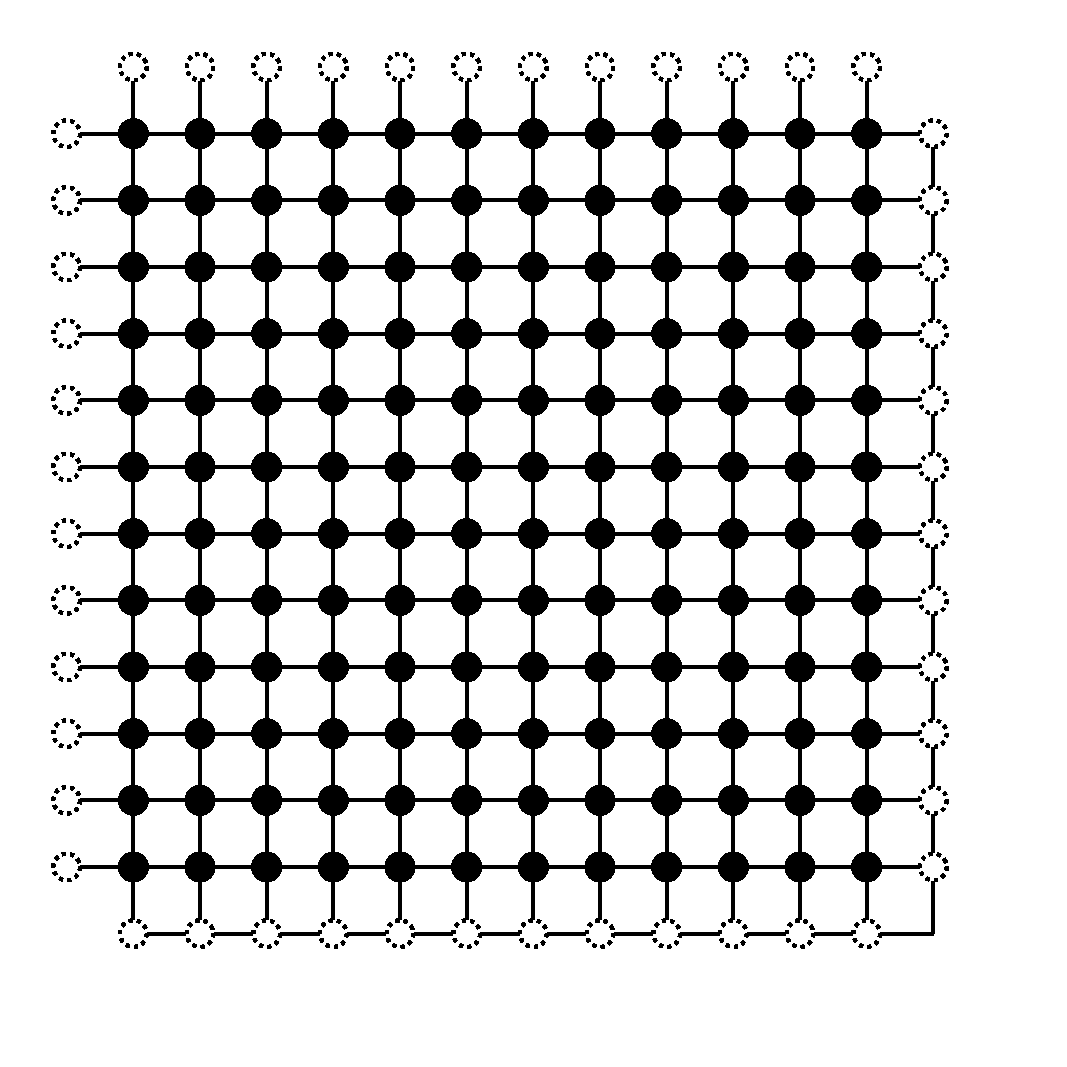
\includegraphics[width=0.30\textwidth]{images/GG/sigma_e0}
            }
            \subfigure[][$\sigma = 0.01$]
            {
                \label{sfig:GG_sigma:0.01}
                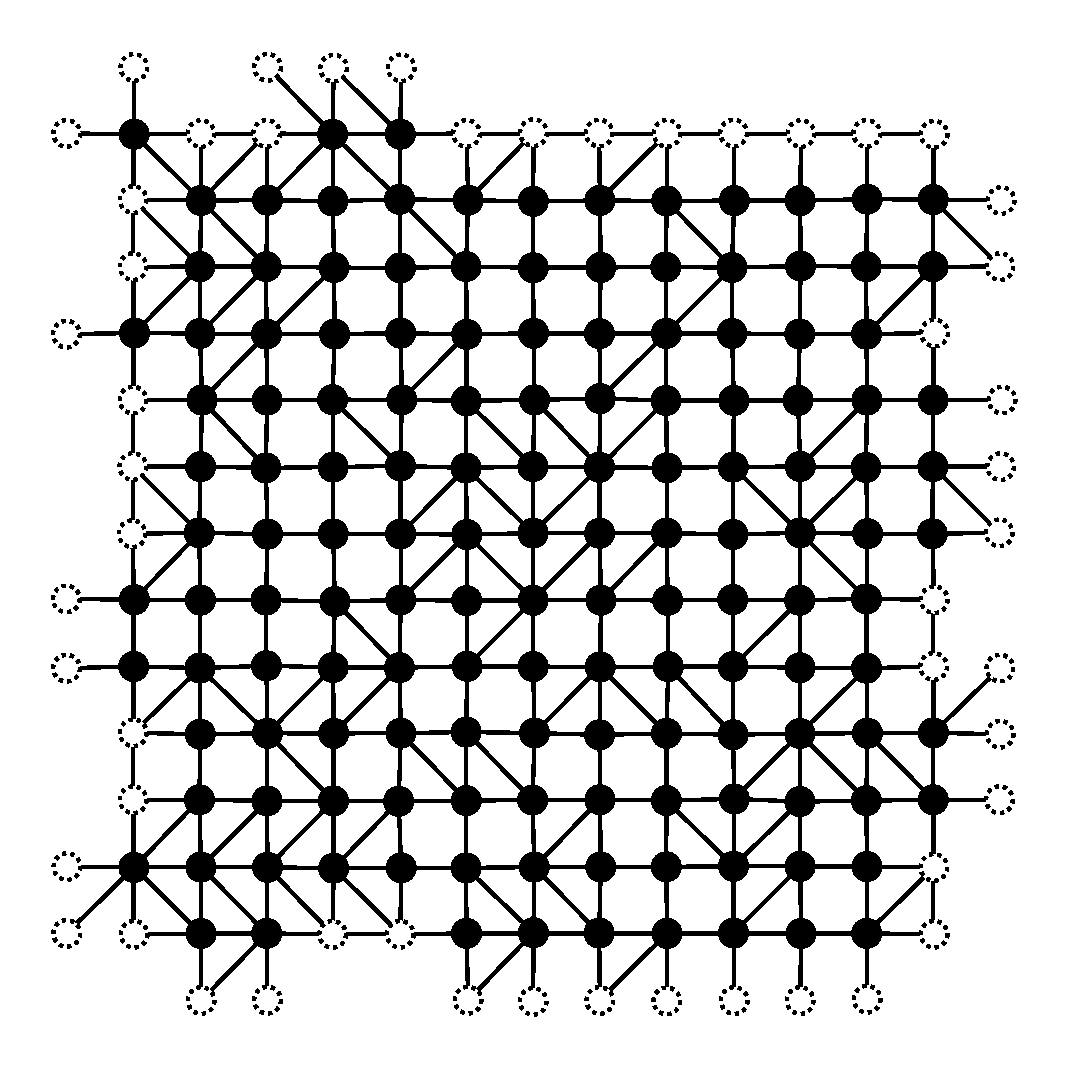
\includegraphics[width=0.30\textwidth]{images/GG/sigma_g0}
            }

            \subfigure[][$\sigma = 0.09$]
            {
                \label{sfig:GG_sigma:0.09}
                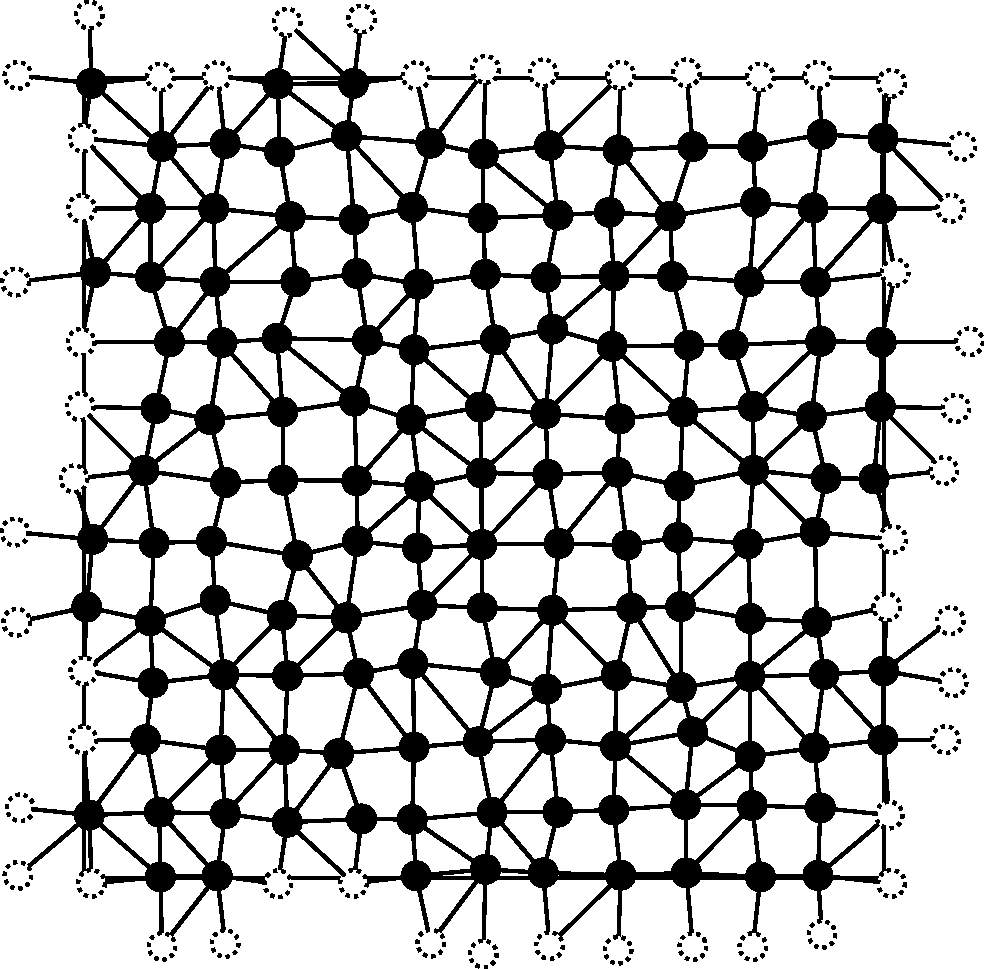
\includegraphics[width=0.30\textwidth]{images/GG/out009}
            }
            \subfigure[][$\sigma = 0.15$]
            {
                \label{sfig:GG_sigma:0.15}
                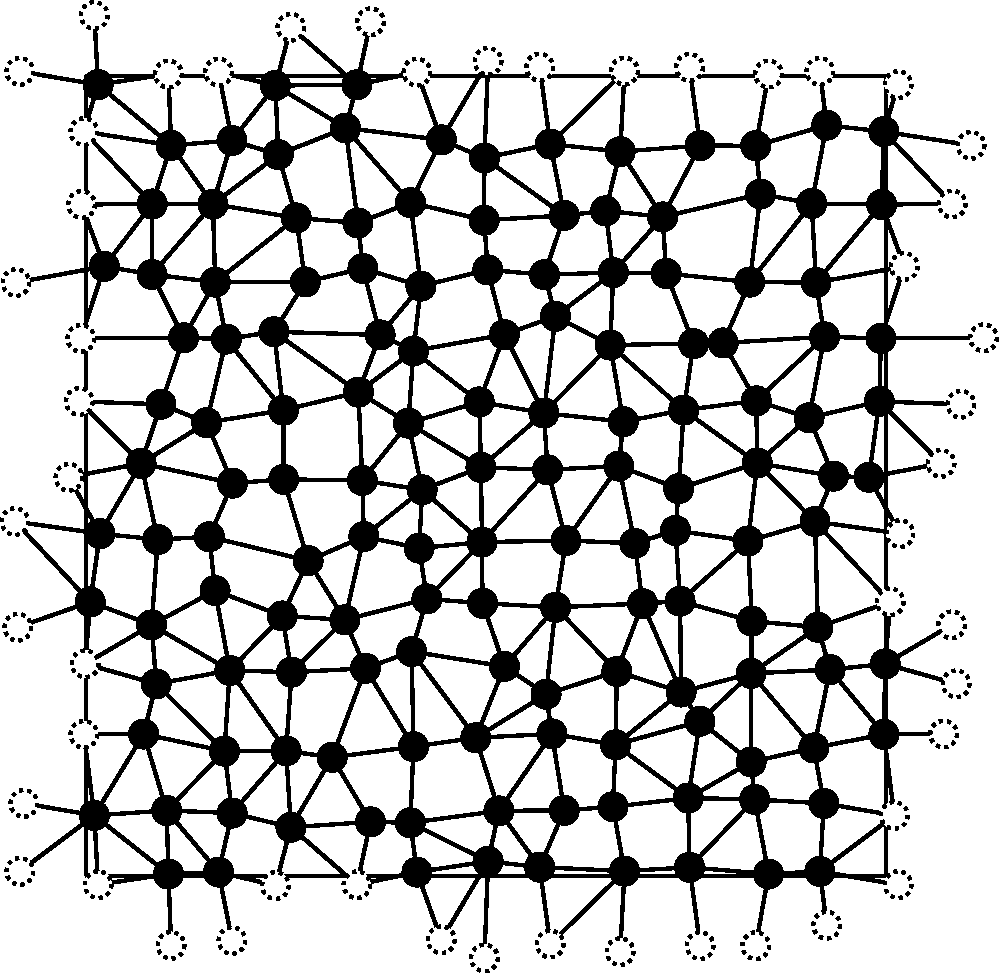
\includegraphics[width=0.30\textwidth]{images/GG/out015}
            }
            \subfigure[][$\sigma = 0.21$]
            {
                \label{sfig:GG_sigma:0.21}
                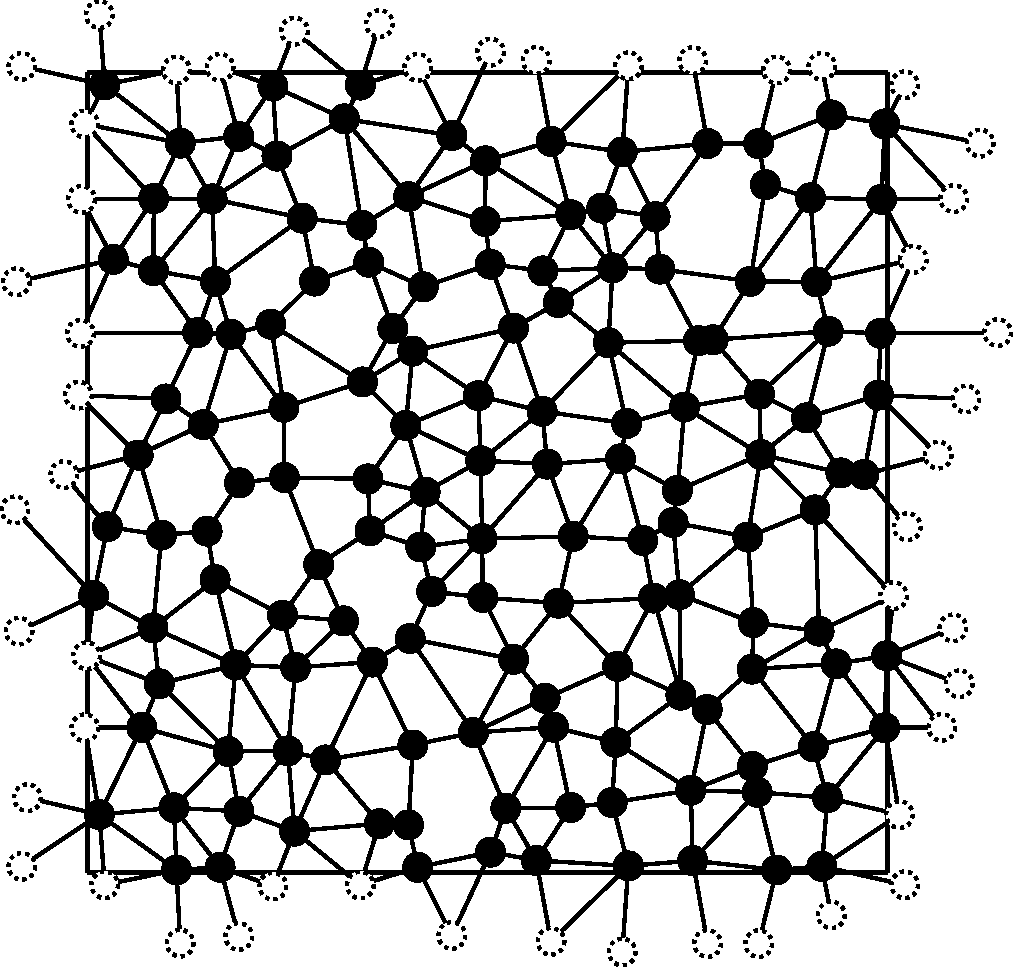
\includegraphics[width=0.30\textwidth]{images/GG/out021}
            }

            \caption[Examples of GG for different $\sigma$]
            {
                GG with periodic boundary conditions for different \(\sigma\).
                The number of edges increases from \subref{sfig:GG_sigma:0.00}
                to \subref{sfig:GG_sigma:0.01} significantly. Until \subref{sfig:GG_sigma:0.15}
                it increases and after that the number of edges decreases.
            }
            \label{fig:GG_sigma}
        \end{figure}\\
        The evolution of the RNG with increasing \(\sigma\) can be made plausible
        with the same arguments. Fig. \ref{fig:RNG_sigma}
        shows that for \(\sigma \lesssim 0.1\) the square lattice character is
        preserved -- no new edges arise and only a few existing edges vanish, which
        explains the plateau in the \(T_{c}\) diagram. With
        increasing \(\sigma\), more and more edges vanish\footnote{See also \url{http://www.youtube.com/watch?v=rltzi15mTM4} for an animation.},
        thus reducing the degree and consequently the corresponding value of \(T_{c}\).
        \begin{figure}[htb]
            \centering
            \subfigure[][$\sigma = 0.09$]
            {
                \label{sfig:RNG_sigma:0.09}
                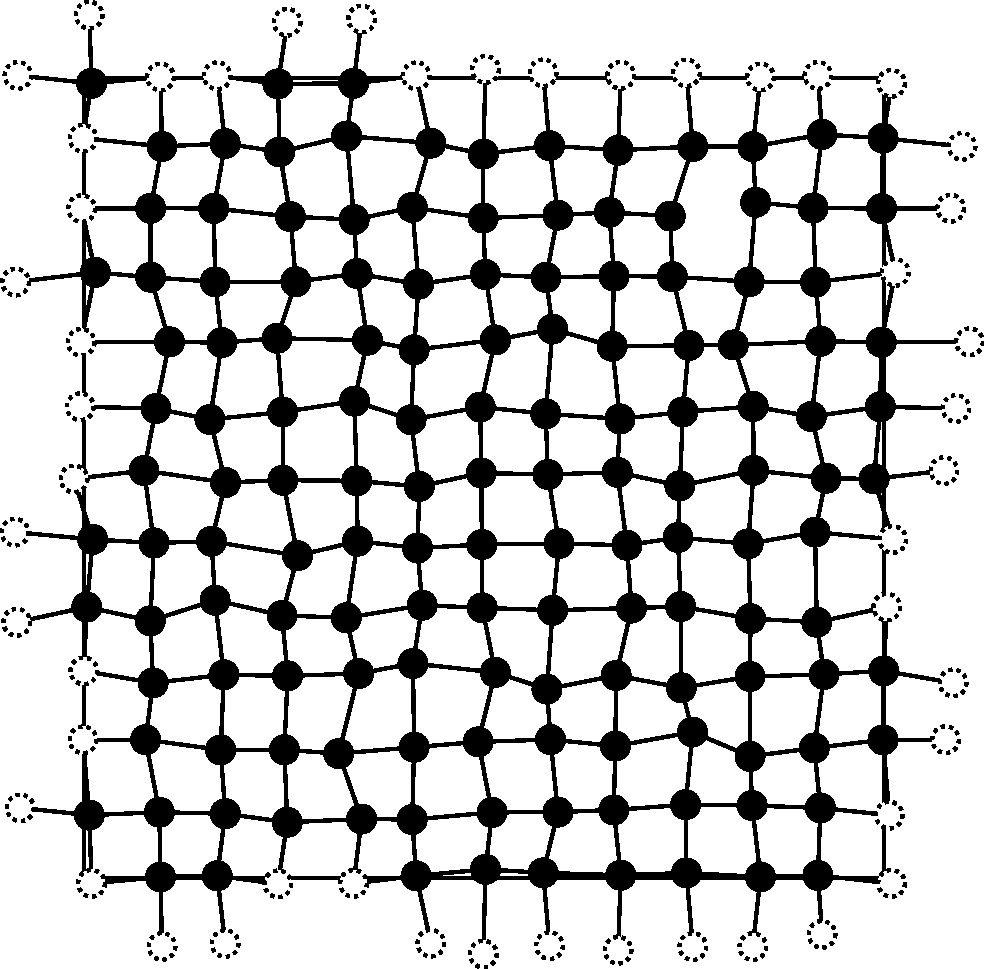
\includegraphics[width=0.30\textwidth]{images/RNG/out009}
            }
            \subfigure[][$\sigma = 0.15$]
            {
                \label{sfig:RNG_sigma:0.15}
                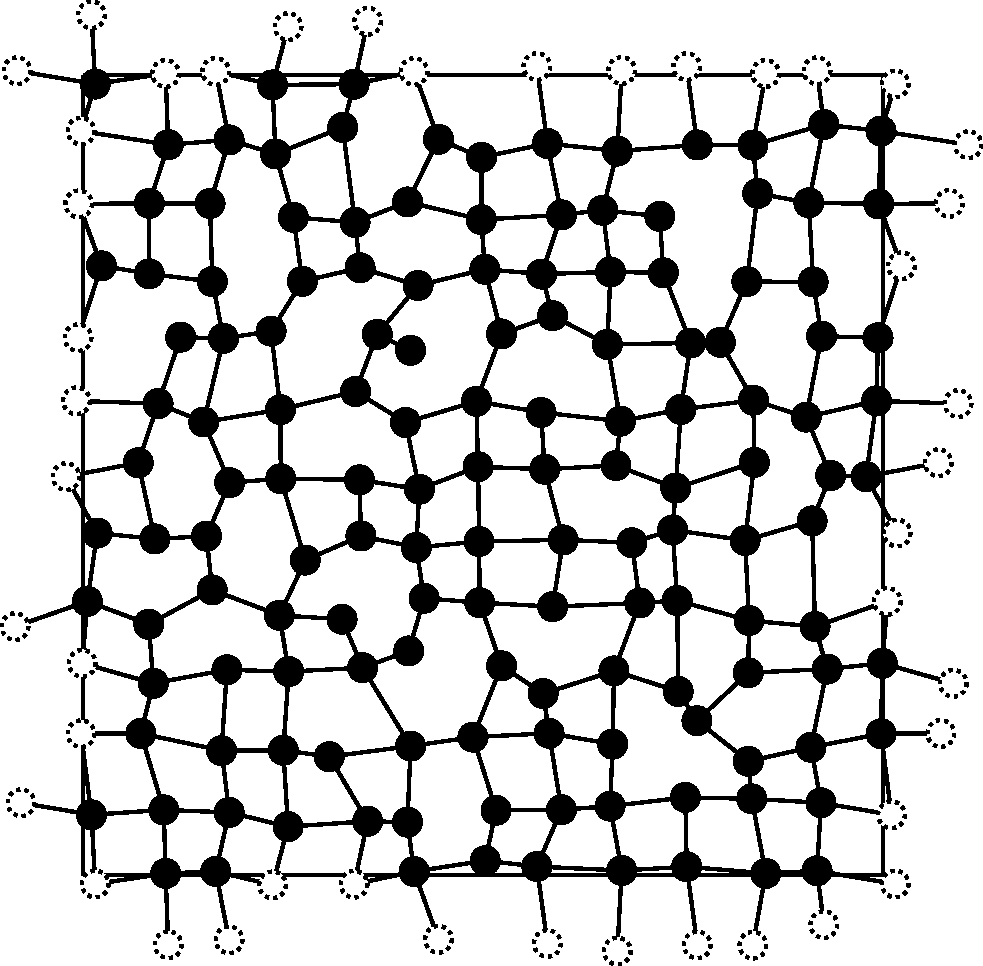
\includegraphics[width=0.30\textwidth]{images/RNG/out015}
            }
            \subfigure[][$\sigma = 0.21$]
            {
                \label{sfig:RNG_sigma:0.21}
                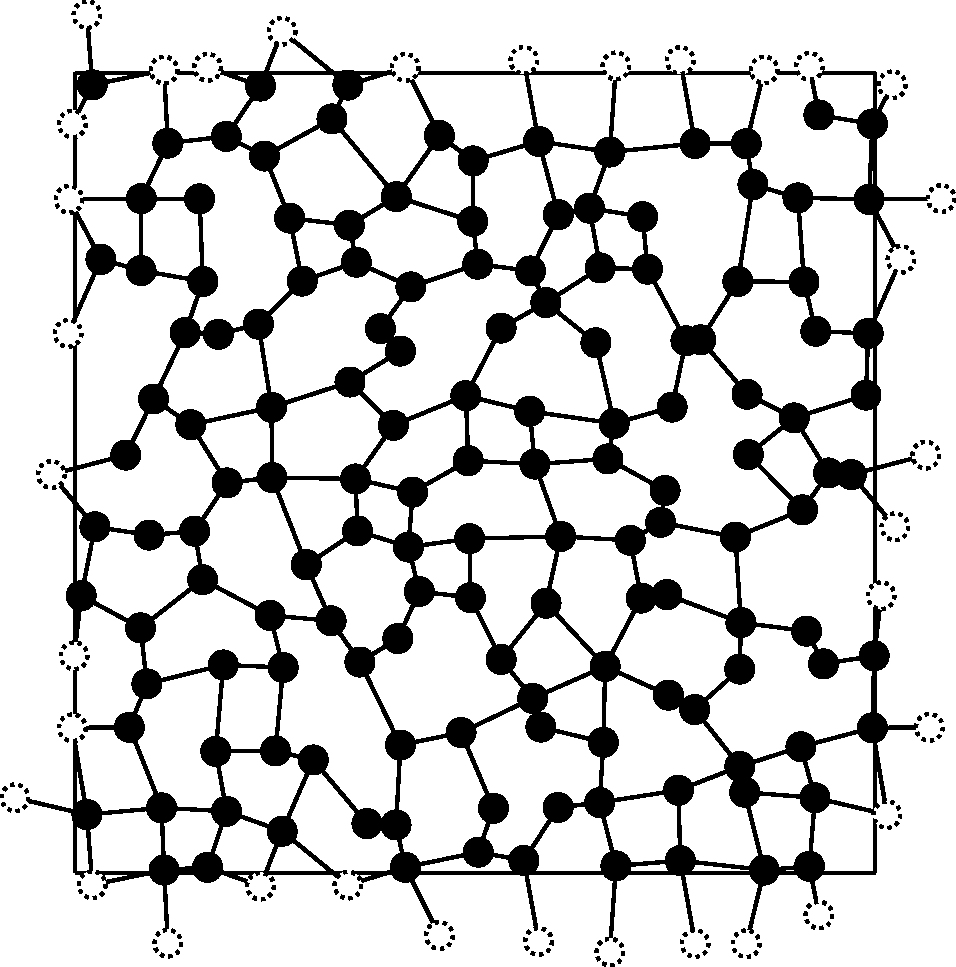
\includegraphics[width=0.30\textwidth]{images/RNG/out021}
            }

            \caption[Examples of RNG for different $\sigma$]
            {
                RNG with periodic boundary conditions for different \(\sigma\).
                \subref{sfig:RNG_sigma:0.09} has still almost the square lattice
                configuration of edges, which is why the plateau from Fig.\ \ref{fig:Tc}\subref{sfig:Tc:RNG}
                exists. In the next two pictures one sees the fast disappearance
                of edges, chracteristic for the RNG for a set of randomly
                distributed points (i.e.\ Poisson process).
            }
            \label{fig:RNG_sigma}
        \end{figure}
        \clearpage

    \subsubsection{Influence of the Coupling Constant on the Critical Temperature}%
    \label{sssec:J}
        However, note that the degree does not alone influence the behavior of \(T_c\).
        Further \(T_c\) depends on the coupling constant \(J_{ij}\), which is
        obvious from Eqs.\ \eqref{eq:exactTc} and \eqref{eq:exactHCTc}. The
        coupling constant in turn is depending on the length of the edges,
        which changes with \(\sigma\).
        Therefore  in Fig.\ \ref{fig:TcJ}\subref{sfig:sumJ:RNG}\subref{sfig:sumJ:GG}
        the mean sum of the coupling constants to all neighbors
        \begin{equation}
            \avg{\sum_{\avg{i,j}} J_{ij}}
        \end{equation}
        is plotted. This is a number which should combine the dependence on
        the degree and the coupling constant. It is determined by summing
        over the edge weights of all edges connected to a node and averaging
        this value over all nodes. Alternatively it is the average edge weight
        of all edges of the graph multiplied by the degree \(\avg{J_{ij}} K\).
        The plot Fig.\ \ref{fig:Tc_J} shows that
        there is a less obvious dependency between \(T_c\) and \(\avg{\sum_{\avg{i,j}} J_{ij}}\)
        than between \(T_c\) and \(K\) (c.f.\ Fig.\ \ref{fig:Tc_K}).
        \begin{figure}[htbp]
            \centering
            \includegraphics[width=0.45\textwidth]{plots/Tc_J}
            \caption[Critical Temperature as a Function of the Degree of the Graph]
            {
                The critical temperature is plotted as a function of the
                average edge weight. The curve shows a less straight line
                than Fig.\ \ref{fig:Tc_K}.
            }
            \label{fig:Tc_J}
        \end{figure}\\
        Though Eq.\ \eqref{eq:exactHCTc} and Fig.\ \ref{fig:Tc_J} show
        that there is no linear connection between \(J\) and \(T_c\), the best guess
        is a linear connection, because this model is derived from the
        square lattice, where the connection is linear. Therefore, one
        normalizes \(T_c\) with \(\avg{\sum_{\avg{i,j}} J_{ij}}\) as in
        Fig.\ \ref{fig:TcJ}\subref{sfig:Tc_normJ:RNG}\subref{sfig:Tc_normJ:GG}, the
        jump on the GG arises again, but \(T_c\) is now monotonically
        decreasing with increasing disorder parameter \(\sigma\).
        \begin{figure}[hbtp]
            \centering
            \subfigure[][]
            {
                \label{sfig:sumJ:RNG}
                \includegraphics[width=0.45\textwidth]{plots/RNG_sumJ}
            }
            \subfigure[][]
            {
                \label{sfig:sumJ:GG}
                \includegraphics[width=0.45\textwidth]{plots/GG_sumJ}
            }

            \subfigure[][]
            {
                \label{sfig:Tc_normJ:RNG}
                \includegraphics[width=0.45\textwidth]{plots/RNG_Tc_normJ}
            }
            \subfigure[][]
            {
                \label{sfig:Tc_normJ:GG}
                \includegraphics[width=0.45\textwidth]{plots/GG_Tc_normJ}
            }

            \subfigure[][]
            {
                \label{sfig:TcD:RNG}
                \includegraphics[width=0.45\textwidth]{plots/RNG_d}
            }
            \subfigure[][]
            {
                \label{sfig:TcD:GG}
                \includegraphics[width=0.45\textwidth]{plots/GG_d}
            }

            \caption[Critical Temperature Normalized by Mean Sum of the Coupling Constants]
            {
                Top: Mean sum of the coupling constants to all
                neighbors over different disorder parameters for
                \subref{sfig:sumJ:RNG} the RNG and
                \subref{sfig:sumJ:GG} the GG.
                Middle: Critical temperatures normalized by mean sum of the
                coupling constants \(\avg{\sum_{\avg{i,j}} J_{ij}}\) over different
                disorder parameters for
                \subref{sfig:Tc_normJ:RNG} the RNG and
                \subref{sfig:Tc_normJ:GG} the GG.
                Bottom: The mean length of all edges \(d\) for
                \subref{sfig:TcD:RNG} RNG
                and \subref{sfig:TcD:GG} GG for different system sizes \(L\)
                averaged over 100 different realizations.
            }
            \label{fig:TcJ}
        \end{figure}\\
        Moreover the forms of both curves are quite similar, but the
        one for the RNG in Fig.\ \ref{fig:TcJ}\subref{sfig:Tc_normJ:RNG}
        is generally lower and spans over a bigger temperature range than
        the curve of the GG in Fig.\ \ref{fig:TcJ}\subref{sfig:Tc_normJ:GG}.
        Both graph types have a plateau at \(0 < \sigma < 0.1\). The conclusion
        is that small disorder has little influence on this normalized critical
        temperature.
        Also both graph types exhibit a steep decline after the plateau before
        they approach an asymptotic limit for \(\sigma \gg 1\).\\
        Although one could assume, that the course of \(\avg{\sum_{\avg{i,j}} J_{ij}}\)
        should be strongly influenced by the mean length of the edges, because \(J_{ij}\)
        is a function on the edge length \(d_{ij}\), this is not exactly the case.
        As shown in Fig.\ \ref{fig:TcJ}\subref{sfig:TcD:RNG}\subref{sfig:TcD:GG}, the
        coarse course is similar but \(d\) shows especially at low \(\sigma\)
        a more complicated course than \(T_c\) and \(\avg{\sum_{\avg{i,j}} J_{ij}}\).
        This is a hint that the influence of \(K\) on \(T_c\) is much more
        important than the influence of \(d\) and therefore the influence
        of \(J_{i,j}\) on \(T_c\). At least with the chosen function for \(J_{ij}\).\\
        If one looks at the behavior of \(\avg{\sum_{\avg{i,j}} J_{ij}}\)
        for \(\sigma \ll 1\) and consequently \(d_{ij} \approx 1\), the
        following approximation is valid.
        \begin{equation}
            \abs{1-d_{ij}} := \varepsilon \ll 1
        \end{equation}
        \begin{equation}
            J_{ij} = e^{\pm \alpha \varepsilon} \approx 1 \pm \varepsilon \mp \dots
        \end{equation}
        \begin{align}
            \avg{\sum_{\avg{i,j}} J_{ij}} &\approx \avg{\sum_{\avg{i,j}} (1 \pm \varepsilon)} \\
                                          &= \frac{1 \pm \varepsilon}{N} \sum_{\avg{i,j}} 1 \\
                                          &= K(1 \pm \varepsilon) \approx K
        \end{align}
        Therefore this normalization is independent of the choice of \(\alpha\)
        at small values of \(\sigma\). In Sec.\ \ref{appendix:fixedCoupling}
        in Fig.\ \ref{fig:Tc_deg_A0}\subref{sfig:Tc_norm_deg:RNG_A0}\subref{sfig:Tc_norm_deg:GG_A0}
        the values from Fig.\ \ref{fig:TcJ}\subref{sfig:Tc_normJ:RNG}\subref{sfig:Tc_normJ:GG}
        are compared to \(T / K\) for \(\alpha = 0\).

    \subsubsection{Course of the Critical Temperature with Fixed Coupling Constants}
    \label{appendix:fixedCoupling}
        A quick analysis of this model with fixed coupling constants \(J = 1\)
        (i.e.\ \(\alpha=0\)) is performed. The results are displayed in Fig.\ \ref{fig:Tc_deg_A0}.
        The jump from \(\sigma=0\) to \(\sigma>0\) does not disappear as in Fig.\ \ref{fig:Tc_deg}
        for variable \(J\) with \(\alpha=0.5\). This suggests that the
        disappearance of the jump is a random special case for the function
        \(J_{ij}=e^{\alpha(1-d_{ij})}\) at \(\alpha=0.5\).\\
        The simulations were carried out on \(L \in \{16,32,64\}\) lattices
        for a subset of the \(\sigma\) and \(T\) used in the previous simulation.
        Also note that the degree \(K\) is
        the same used in \ref{fig:Tc}\subref{sfig:deg:RNG}\subref{sfig:deg:GG}
        because it is obviously independent of \(J\).
        Further, note that for small values of \(\sigma\), \(T_c / K\)
        obtained using the fixed coupling strength \(J=1\) coincides with
        \(T_c / \avg{\sum_{\avg{i,j}}J_{ij}}\) obtained using the distance
        dependent coupling strength (see Eq.\ \ref{eq:coupling}).
        This can be expected from the approximate analytic statement presented
        in Sec.\ \ref{sssec:J}.
        \begin{figure}[htb]
            \centering
            \subfigure[][]
            {
                \label{sfig:Tc:RNG_A0}
                \includegraphics[width=0.45\textwidth]{plots/RNG_Tc_A0}
            }
            \subfigure[][]
            {
                \label{sfig:Tc:GG_A0}
                \includegraphics[width=0.45\textwidth]{plots/GG_Tc_A0}
            }

            \subfigure[][]
            {
                \label{sfig:Tc_norm_deg:RNG_A0}
                \includegraphics[width=0.45\textwidth]{plots/RNG_Tc_norm_deg_A0}
            }
            \subfigure[][]
            {
                \label{sfig:Tc_norm_deg:GG_A0}
                \includegraphics[width=0.45\textwidth]{plots/GG_Tc_norm_deg_A0}
            }

            \caption[Critical Temperature and Critical Temperature Normalized by Degree of the Graph for Fixed Coupling Constants $J=1$]
            {
                Top: Critical Temperature \(T_c\) of the graph over different
                disorder parameters \(\sigma\) with fixed coupling constants \(J=1\) for
                \subref{sfig:deg:RNG} the RNG and
                \subref{sfig:deg:GG} the GG.
                Bottom: Critical temperatures normalized by degree \(K\) over
                different disorder parameters \(\sigma\) with fixed coupling constants \(J=1\) for
                \subref{sfig:Tc_norm_deg:RNG} the RNG and
                \subref{sfig:Tc_norm_deg:GG} the GG. The values of \(T_c / K\)
                are compared to those of \(T_c /  \avg{\sum_{\avg{i,j}}J_{ij}}\)
                from Sec.\ \ref{sssec:J}.
            }
            \label{fig:Tc_deg_A0}
        \end{figure}\\
        Ref.\ \cite{Janke1994} gives a critical temperature for the DT with \(J=1\)
        \(T_{c,DT} = 3.80\)\footnote{more precise: a value of \(\frac{1}{T_c} \approx 0.263\) is given}.
        It can be compared to the obtained \(T_{c,GG} = 2.19\)
        and \(T_{c,RNG} = 1.13\) for \(\sigma = 1.2\), which should
        ensure a set of nodes very similar to a Poisson process.
        Note that while for the graph ensembles the relation
        \begin{equation}
            DT \supseteq GG \supseteq RNG
        \end{equation}
        holds (see Sec. \ref{ssec:graphtypes}), the relation for the
        critical points on these graphs
        \begin{equation}
            T_{c,DT} \ge T_{c,GG} \ge T_{c,RNG}
        \end{equation}
        is also true.
        Also keep in mind that the relation \(T_{c,GG} \ge T_{c,RNG}\)
        was true for \(\alpha = 0.5\) in the preceding sections.
        This phenomenon is also known from percolation where the relation
        \(p_{c,DT} \ge p_{c,GG} \ge p_{c,RNG}\) holds for the percolation
        threshold \(p_c\) -- the critical point of the percolation problem.
        The fact that the subgraph hierachy can be translated to
        the sequence of \(p_c\) for the subgraphs, is known as the containment
        theorem \cite{fisher}.
        Possibly the containment theorem is also applicable on this kind of
        problem.

\subsection{Critical Value of the Binder Cumulant}
    The value of the Binder cumulant at the critical point \(g_c\)
    depends strongly on boundary conditions but only weakly on the precise lattice
    structure \cite{BinderValue}. For periodic boundary conditions on a
    square lattice it is \(g_c \approx 0.916\) according to \cite{BinderValue}
        \footnote{Note that \cite{BinderValue} uses another definition of
            the Binder cumulant, and has to be normalized by \(\frac{2}{3}\)
            to match the definition in this thesis.}.
    Because the analysis of Sec.\ \ref{ssec:binderIntersections}
    yields \(g_c\) anyway, it is easy to check the consistency and
    behavior of \(g_c\) in the geometrically disordered Ising model.
    The error bars are the standard error of the six values obtained
    through the intersections.\\
    \begin{figure}[htbp]
        \centering
        \subfigure[for a RNG][]
        {
            \label{sfig:TcG:RNG}
            \includegraphics[width=0.45\textwidth]{plots/RNG_TcG}
        }
        \subfigure[for a GG][]
        {
            \label{sfig:TcG:GG}
            \includegraphics[width=0.45\textwidth]{plots/GG_TcG}
        }
        \caption[Values of the Binder Cumulant at the Critical Point $g_c$]
        {
            Values of the Binder cumulant at the critical point \(g_c\)
            for
            \subref{sfig:TcG:RNG} a RNG and
            \subref{sfig:TcG:GG} a GG for different \(\sigma\).
            The dotted line is the reference value for square lattices
            with periodic boundary conditions \cite{BinderValue}, which
            corresponds to \(\sigma = 0\).
        }
        \label{fig:TcG}
    \end{figure}\\
    Considering both plots in Fig.\ \ref{fig:TcG}, \(g_c\) is for low
    \(\sigma\) obviously always bigger than the known value. Though the
    deviations are only very small. Perhaps this overestimation is caused
    by the cubic spline interpolation used to acquire these \(g_c\) values.
    Or this are again finite size effects which would disappear for
    larger system sizes.
    For bigger \(\sigma\) the uncertainty gets greater, but the values
    do only differ by a few percent, hence even the big disorder and
    definition of nearest neighbors via a proximity graph does not change
    the value of \(g_c\) much. Though it is mentioned in \cite{BinderValue} that the
    lattice structure has a minor effect on \(g_c\), the uncertainty of
    \(g_c\) is too large to confirm this. For a more exact analysis, new
    Monte Carlo simulations at \(T_c\) would be needed. But this is
    beyond the scope of this thesis. Anyway, the results show the expected
    behavior, because no major deviations from the value of \(g_c\) at
    \(\sigma = 0\) occur at larger \(\sigma\). Within error bars the
    values are all in reasonable agreement with \(g_c\).


    \section{Conclusion}
        \label{sec:conclusion}
This study shows that universality of the Ising model is preserved for
irregular graphs on a wide range of configurations which are intermediate
between the square lattice Ising model and a random Poisson point process.
Also the critical temperature was measured over this range and determined
that it shows approximately a power law behavior with the mean
number of neighbors as the base and an exponent dependent on the
graph type that defines the neighbor relationships.

The next step would be the extension to three and higher
dimensions, where the used proximity graphs are still well defined. It
would also be worthwhile to study properties of the graph ensembles themselves,
because -- to our knowledge -- they are mostly studied in 2D \cite{RNGCell}.


    \clearpage
    \bibliography{lit}
    \bibliographystyle{alpha}
    %~ \bibliographystyle{amsplain}

    \clearpage
    \begin{appendix}
        \section{Finite Size Effects at the Example of the Specific Heat}
\label{appendix:finiteSizeEffects}
    In fig. \ref{fig:smeared_out_appendix} the specific heat
    \[C = \frac{N}{T^2}\avg{\avg{E^2} - \avg{E}^2}\]
    is plotted for different system sizes. The finite size effects are obvious.
    The divergence is finite, and gets shallower with smaller \(L\). Besides
    the maximum moves away from the critical temperature with smaller \(L\).
    \begin{figure}[htbp]
        \centering
        \includegraphics[width=0.45\textwidth]{plots/Specific_Heat_0}
        \caption[Finite Size Effects by Example of the Specific Heat]
        {
            Effects of different system sizes at \(\sigma = 0\). Dotted lines
            are guides to the eye.
        }
        \label{fig:smeared_out_appendix}
    \end{figure}

\section{Finite Size Scaling at the Example of the Susceptibility and Magnetisation}
\label{appendix:finiteSizeScaling}
    In fig. \ref{fig:gettingCrit:appendix}\subref{sfig:gettingCrit:s_0_sus}
    the magnetic susceptibility
    \[\chi = \frac{1}{TN}\avg{\avg{m^2} - \avg{m}^2}\]
    is plotted and in \ref{fig:gettingCrit:appendix}\subref{sfig:gettingCrit:collapse_s_0_sus}
    collapsed to determine the critical exponent \(\beta\).
    Analog for the mean absolute magnetisation \(\avg{\abs{m}}\) in fig \ref{fig:gettingCrit:appendix}
    \subref{sfig:gettingCrit:s_0_meanM}\subref{sfig:gettingCrit:collapse_s_0_meanM}
    to determine the critical exponent \(\gamma\).
    Both are at \(\sigma=0\) and
    both collapses reproduce the  critical exponent \(\nu\) and the
    critical temperature \(T_c\) in good agreement with the before determined
    values from fig. \ref{fig:gettingCrit}\subref{sfig:gettingCrit:collapse_s_0}
    and the analytically known values. This is a good cross check
    for consistency.
    \begin{figure}[htbp]
        \centering
        \subfigure[Susceptibility $\chi$][]
        {
            \label{sfig:gettingCrit:s_0_sus}
            \includegraphics[width=0.47\textwidth]{plots/s_0_sus}
        }
        \subfigure[Finite Size Scaling of the Susceptibility $\chi$][]
        {
            \label{sfig:gettingCrit:collapse_s_0_sus}
            \includegraphics[width=0.47\textwidth]{plots/collapse_s_0_sus}
        }
        \subfigure[Magnetisation $\avg{\abs{m}}$][]
        {
            \label{sfig:gettingCrit:s_0_meanM}
            \includegraphics[width=0.47\textwidth]{plots/s_0_meanM}
        }
        \subfigure[Finite Size Scaling of the Magnetisation $\avg{\abs{m}}$][]
        {
            \label{sfig:gettingCrit:collapse_s_0_meanM}
            \includegraphics[width=0.47\textwidth]{plots/collapse_s_0_meanM}
        }
        \caption[Examples of determining critical temperature and exponents]
        {
            Examples for finite size scaling.
        }
        \label{fig:gettingCrit:appendix}
    \end{figure}

    \end{appendix}

    \clearpage
    \pagestyle{empty}
    


    \cleardoublepage
    \selectlanguage{ngerman}
    \thispagestyle{empty}
\addcontentsline{toc}{section}{Erkl\"{a}rung}
Hiermit versichere ich, dass ich diese Arbeit selbstständig verfasst und
keine anderen als die angegebenen Quellen und Hilfsmittel benutzt habe.
Außerdem versichere ich, dass ich die allgemeinen Prinzipien
wissenschaftlicher Arbeit und Veröffentlichung, wie sie in den
Leitlinien guter wissenschaftlicher Praxis der Carl von Ossietzky
Universität Oldenburg festgelegt sind, befolgt habe.\\[3cm]

\raggedleft
\hfill Oldenburg den \today, ..............................................\\
\hfill (Hendrik Schawe)\\


\end{document}
